% ============================================================
% Consolidated Appendix
% ============================================================
\newpage
\appendix

% ============================================================
\section{Extended Limitations and Future Work}
\label{app:limitations}
% (Summary in main body, \S\ref{sec:limitations}.)
% ============================================================

\textbf{(1) Single-backbone scope of the dissociation claim.}
The drift--utility dissociation is established on the \emph{Moirai
family} only (Small 13.8M, Base 91M, Large 311M across ETTh1, ETTh2,
ETTm2).  We attempted three further backbones as second-model
controls across three ETT datasets (Table~\ref{tab:backbone_screen}).

\begin{table}[ht]
\centering\small
\caption{The initial non-Moirai screen, at $h{=}96$ with a lookback of $192$, one
seed (42) and $300$ test windows. \textbf{This is a different protocol from the
paper's non-Moirai screen} (Table~\ref{tab:crossbackbone}), which runs $h{=}24$
at lookback~$96$ with three seeds and a paired frozen-encoder condition; the two
are therefore not comparable cell by cell, and only the latter feeds the 32-cell
count. Chronos-T5-Base/Large and MOMENT appear here and nowhere else. Advantage
is $R^2_\text{task}(\text{PT})$ as a percentage. Rows trace to
\texttt{results/v10\_chronos\_etth2.json}, \texttt{v14\_*}, \texttt{v18\_backbone\_gate/*}
and \texttt{v12\_moment\_etth2\_gate.json}.}
\label{tab:backbone_screen}
\begin{tabular}{llccc}
\toprule
Backbone & Dataset & ZS MSE & Linear MSE & Advantage \\
\midrule
Chronos-T5-Small  & ETTh2 & 0.304 & 0.213 & $-$42.6\% \\
Chronos-T5-Small  & ETTh1 & 0.118 & 0.092 & $-$28.8\% \\
Chronos-T5-Small  & ETTm2 & 0.188 & 0.110 & $-$70.2\% \\
Chronos-T5-Base   & ETTh2 & 0.286 & 0.213 & $-$34.3\% \\
Chronos-T5-Large  & ETTh2 & 0.288 & 0.213 & $-$35.2\% \\
TimesFM-2.5-200M  & ETTh2 & 0.242 & 0.213 & $-$13.8\% \\
TimesFM-2.5-200M  & ETTh1 & 0.105 & 0.092 & $-$13.9\% \\
TimesFM-2.5-200M  & ETTm2 & 0.190 & 0.110 & $-$72.6\% \\
MOMENT-1-base     & ETTh2 & 0.528 & 0.213$^{*}$ & $-$148\%  \\
\bottomrule
\end{tabular}

\vspace{2pt}
{\footnotesize $^{*}$MOMENT was screened at lookback~$96$, whose baseline is
$0.235$; its margin was nonetheless computed against the lookback-192 baseline
$0.213$, and we print the comparator actually used. Against $0.235$ the margin is
$-125\%$, so the verdict is unchanged either way.}
\end{table}

All nine backbone$\times$dataset cells gate-fail (ZS under-performs
the Linear baseline by 14\% to 148\%), consistent with ETT-family
distributions being outside the pre-training coverage of these
backbones at these sizes.  The Chronos capacity sweep
(Chronos-T5-Small/Base/Large on ETTh2) confirms the gap is
size-invariant: scaling from Small (210M) to Large (710M)
yields no improvement ($-$42.6\% $\to$ $-$34.3\% $\to$ $-$35.2\%).
TimesFM-2.5-200M and MOMENT-1-base gate-fail across all tested datasets.
We interpret this pattern as a substantive finding about
\emph{backbone-specific ETT coverage} rather than evidence against
generality of the dissociation: matched-protocol ZS under-performance
on a value-gate design means fine-tuning these backbones on ETT
cannot meaningfully distinguish drift-as-forgetting from
drift-as-adaptation (there is no valuable feature to forget).  A
gate-passing second backbone on a different dataset (Traffic, ILI,
Exchange, or a model with explicit ETT pre-training coverage)
remains the most direct path to a multi-backbone replication and
is the highest-priority future-work direction.

\textbf{(2) Sample-sweep depth and seed count.}
The central sample-size sweep (Table~\ref{tab:sample_sweep}) covers
ETTh2 at $n \in \{500, 1\text{k}, 2\text{k}, 5\text{k}, 10\text{k}\}$.
At $n{=}10$k we report the CUDA 10-seed deterministic early-stopped result:
$k{=}10$ seeds (42, 101, 123, 202, 303, 456, 777, 789, 888, 999),
all completed (no NaN); \texttt{--deterministic} flag
(\texttt{CUBLAS\_WORKSPACE\_CONFIG=:4096:8}, \texttt{cudnn.deterministic=True},
seeded DataLoader, PYTHONHASHSEED).
Forg.\ $-$5.3$\pm$6.6\%, 7/10 negative; mean best epoch $4.2{\pm}1.3$.
The Ridge $\Delta R^2{=}{+}$0.67$\pm$0.24 (\textbf{10/10} positive) that an
earlier version reported alongside these is \textbf{retracted}
(\S\ref{sec:retraction}) and is quoted here only as a record of the withdrawn
computation; the forgetting and CKA columns are unaffected.
The three near-zero positive-forgetting seeds (123: $+$1.8\%, 456: $+$4.4\%, 789: $+$0.4\%)
follow the $n{=}5$k overshoot pattern (Fig.~\ref{fig:dissociation}, right panel).
For comparison, MPS early-stopped $k{=}10$ gave $-$5.7$\pm$10.4\% (8/10 neg,
\texttt{v18\_mps\_deterministic\_n10k}); a second early-stopped run ($k{=}5$) gave
$-$11.7$\pm$5.3\% (all 5 negative, \texttt{v17\_etth2\_n10k\_es}); the
final-epoch runs, the only ones without early stopping, gave
$+$10.6$\pm$9.8\% on $k{=}3$ (\texttt{v16\_etth2\_n10k}), which is the
protocol dependence \S\ref{sec:analysis} discusses.
Moirai-Base is now evaluated at both $n{=}500$ and $n{=}10$k (10 seeds each);
full $n$-sweep on Moirai-Large is future work.

\textbf{(3) Probe-head capacity.}
Ridge and MLP absolute $R^2(\text{FT})$ remains negative on the
96-step-ahead head at all sampled $n$, which is exactly why the
$\Delta R^2$ axis is \textbf{retracted} (\S\ref{sec:retraction}): relative
movement between two fits that never decode the target is not evidence about
the encoder. The probe-design sweep of Appendix~\ref{app:noisefloor} shows
only that the direction is stable across $\alpha$, pooling and probe seed
\emph{within} that failed-fit regime; it does not rescue the statistic, and no
claim in this paper rests on it. Probe capacity is therefore no longer a
limitation of a live result but a diagnosis of a withdrawn one.

\textbf{(4) Sample-sweep on other sizes.}
Moirai-Large is evaluated at $n{=}500$ only; full $n$-sweep is future work.
\textbf{(5) IoT scope.}
IoT is a negative control (ZS AUC 0.481, sub-random); fine-tuning replaces
rather than preserves pre-trained features.
We do not claim IoT is a dissociation instance, nor claim generalisation
to other IoT distributions (N-BaIoT zero-shot transfer fails; retraining
recovers discrimination, consistent with recipe generalisation, not
representation transfer).

% ============================================================
\section{uni2ts PackedStdScaler Patch Details}
\label{app:scaler_patch}
% ============================================================

We identified and patched an in-place tensor mutation in
\texttt{uni2ts}'s \texttt{PackedStdScaler} that silently detaches
autograd on losses depending on scaled statistics.  The issue arises
when \texttt{PackedStdScaler.transform} performs an in-place
\texttt{.copy\_()} that breaks the gradient tape.  Our patch replaces
the in-place write with a differentiable \texttt{torch.where}
operation.  \emph{All} Moirai fine-tuning results in this paper use
the patched scaler (released with our code); unpatched
\texttt{uni2ts} runs may converge differently and we have observed
silent non-convergence on \texttt{uni2ts@main}.  We recommend
upstreaming this patch to \texttt{uni2ts}.

% ============================================================
\section{Moirai Median Forecast Selection}
\label{app:moirai_median}
% ============================================================

Moirai generates probabilistic forecasts as a mixture of
distributions (StudentT, NormalFixedScale, NegativeBinomial,
LogNormal).  The heavy-tailed components (NegBin, LogNormal) produce
extreme right-tail outliers when using the \emph{mean} of forecast
samples as the point prediction; for ETTh2 at $h{=}192$, sample
means reached 21{,}431 against a target maximum of 45.5, inflating
MSE from 0.30 to 8.58.

We use the \emph{median} of 20 forecast samples as the robust point
prediction, consistent with the Moirai paper's evaluation protocol.
This eliminates sensitivity to the heavy-tailed mixture components
while preserving the distributional forecast's central tendency.

% ============================================================
\section{ETTh2 Forecasting Details}
\label{app:etth2_details}
% ============================================================

\textbf{Dataset.}
ETTh2 (Electricity Transformer Temperature, Hourly, dataset 2)
contains 17{,}420 timesteps of 7 features (HUFL, HULL, MUFL, MULL,
LUFL, LULL, OT) recorded hourly from electrical transformers.
We use the standard chronological split: 12 months training,
4 months validation, 4 months test.

\textbf{Training protocol.}
For NLL training, we concatenate context (96 timesteps) and target
(96 or 192 timesteps) as input to Moirai's \texttt{\_val\_loss}
with fixed patch size 32.
For evaluation, we use extended lookback sequences
(context\_length $+$ prediction\_length timesteps) with
\texttt{patch\_size='auto'} and take the median of 20 forecast samples.
All data is fed to Moirai in raw scale (Moirai's internal
PackedStdScaler handles instance normalization); predictions and targets
are then normalized using training-set mean and standard deviation
for MSE/MAE computation, matching the standard time-series forecasting
evaluation protocol.

\textbf{Temporal contrastive labels.}
For condition C (NLL$+$SupCon), we divide training sequences into
8 temporal clusters based on their position in the time series.
Sequences within the same cluster are positive pairs; sequences from
different clusters are negatives.
This encourages the encoder to maintain temporal-regime awareness.

\textbf{Horizon selection.}
We evaluate $h{=}96$ and $h{=}192$, the two horizons at which Moirai-Small on
ETTh2 clears the value gate: measured against the fitted lookback-96 baseline
the gate is defined with (Appendix~\ref{app:gatecorrection}),
$R^2_\text{task}(\text{PT}){=}{+}0.400$ at $h{=}96$ and ${+}0.464$ at
$h{=}192$ on held-out windows.
Horizons $h{=}336$ and $h{=}720$ exceed Moirai-Small's
\texttt{max\_seq\_len}$=$512 constraint when combined with the
required extended lookback and are omitted.

% ============================================================
\section{ETTh2 Drift Diagnosis and Mitigation (Full Tables)}
\label{app:full_tables}
% ============================================================

This section contains the full tables referenced in \S\ref{sec:forecasting}.
Table~\ref{tab:mitigation_spectrum} shows the mitigation spectrum, conditions~B
through~H on Moirai-Small/ETTh2 at both horizons. An earlier version also
printed a three-row B/C/D subset of that table separately, with a caption
asserting that Moirai's $28\%$ and $45\%$ zero-shot margins over ``Linear''
confirmed the pre-trained features were valuable; those margins were measured
against the superseded trend baseline (Appendix~\ref{app:gatecorrection}), and
the subset is dropped rather than recaptioned since every row it carried
appears here.

% GENERATED by scripts/emit_r2task.py from results/gate_val_side.json and results/gate_test_side.json -- do not hand-edit.
% The corrected fitted-baseline gate: scripts/gate_all_cells.py --baseline fitted, on both
% splits (300 matched selection windows, 300 matched held-out windows).
% Superseded trend-baseline values are preserved in
% results/gate_test_side_trend.json / results/gate_val_side_trend.json and are not read here.
\begin{table}[t]
\centering
\caption{Baseline-relative pre-trained advantage $\Vb{\text{ridge}} {=} 1 {-}
\text{MSE}_{\text{ZS}}/\text{MSE}_{\text{Linear}}$ for every Moirai cell, on both
splits. The \emph{selection} columns are the paper's primary gate: they are disjoint from
the held-out windows every intervention outcome is scored on, so cell inclusion is not a
judgement made after seeing the outcome. The \emph{held-out} columns are the retrospective
variant, reported as a sensitivity analysis. Bold marks a pass on the \emph{primary} split
in both columns of that row, so the bold set is the one the body's counts refer to.
\textbf{Not a linear probe}: this is a ratio of forecast MSEs computed through
Moirai's own forecasting head, and is unaffected by the retraction of the
linear-probe $\Delta R^2$ axis.
\textbf{Estimator, exactly}: $\text{MSE}_{\text{ZS}}$ is the median of 20
Moirai forecast samples at extended lookback (context $+$ horizon);
$\text{MSE}_{\text{Linear}}$ is a single lookback-96 ridge-OLS linear map
$\mathbb{R}^{96 \times D} {\to} \mathbb{R}^{h \times D}$ \emph{fit on the
cell's training windows} and applied unchanged out of sample; both are computed
on the same matched windows within a split (300 selection, 300
held-out), train-normalised.
The gate involves no fine-tuning, so a cell has one value at every $n$: the
$n{=}500$ and $n{=}10$k (ES) operating points reported in
\S\ref{sec:forecasting} share the entry shown here.
Bold ${=}$ gate-pass at the $0.20$ threshold on the primary split. ``---'' ${=}$ not run.}
\label{tab:r2task}
\small
\begin{tabular}{ll cc cc}
\toprule
& & \multicolumn{2}{c}{Selection (primary)} & \multicolumn{2}{c}{Held-out (retrosp.)} \\
\cmidrule(lr){3-4}\cmidrule(lr){5-6}
Backbone & Dataset & $h{=}96$ & $h{=}192$ & $h{=}96$ & $h{=}192$ \\
\midrule
\multicolumn{6}{l}{\textit{Moirai-Small}} \\
 & ETTh1                  & $-$0.177 & $-$0.347 & $-$0.243 & $-$0.331 \\
 & ETTh2                  & $\mathbf{+0.874}$ & $\mathbf{+0.932}$ & $\mathbf{+0.400}$ & $\mathbf{+0.464}$ \\
 & ETTm2                  & $-$0.164 & $\mathbf{+0.352}$ & $-$0.110 & $\mathbf{+0.108}$ \\
 & Weather                & $-$0.546 & $-$0.506 & $-$0.867 & $-$0.639 \\
 & \texttt{Electricity7}  & $-$0.650 & $-$0.455 & $-$0.085 & $-$0.047 \\
\midrule
\multicolumn{6}{l}{\textit{Moirai-Base}} \\
 & ETTh1                  & $-$0.312 & $-$0.600 & $-$0.458 & $-$0.501 \\
 & ETTh2                  & $\mathbf{+0.777}$ & $\mathbf{+0.925}$ & $\mathbf{+0.361}$ & $\mathbf{+0.275}$ \\
 & ETTm2                  & $-$0.257 & $\mathbf{+0.211}$ & $-$0.057 & $\mathbf{+0.083}$ \\
 & Weather                & $-$0.823 & $-$0.633 & $-$1.029 & $-$1.324 \\
\midrule
\multicolumn{6}{l}{\textit{Moirai-Large}} \\
 & ETTh1                  & $-$0.248 & --- & $-$0.454 & --- \\
 & ETTh2                  & $\mathbf{+0.875}$ & --- & $\mathbf{+0.219}$ & --- \\
 & Weather                & $-$0.638 & --- & $-$0.621 & --- \\
\bottomrule
\end{tabular}
\vspace{1pt}

{\footnotesize
\textbf{Reading:} seven of these 21 cells clear the $0.20$ threshold on the selection windows and five on the held-out windows.
The selection set contains the held-out set and adds two (ETTm2, ETTm2), so the retrospective variant is the stricter of the two here.
The primary survivors span two datasets: ETTh2, ETTm2.
$\Vb{\text{ridge}}{<}0$ means the linear baseline wins outright.
These values supersede the ones printed in earlier versions of this table,
which were computed against a per-window trend extrapolation rather than the
fitted regression the gate is defined with; the substitution and its
consequences are documented in Appendix~\ref{app:gatecorrection}.
\texttt{Electricity7} is Electricity restricted to 7 of its 370 series (six
\texttt{MT} series plus \texttt{OT}), a deliberate protocol deviation that
keeps the cell dimensionality-matched to ETT/Weather.}
\end{table}


Table~\ref{tab:sample_sweep} gives the sample-size sweep on ETTh2
($h{=}96$, condition~B) referenced in \S\ref{sec:forecasting}; its two
$\Delta R^2$ columns are retracted (\S\ref{sec:retraction}) and only the MSE,
Forg.\% and CKA columns should be read.

\begin{table}[t]
\centering
\caption{Sample-size sweep on ETTh2 ($h{=}96$, condition~B).
Drift grows monotonically (CKA$\downarrow$ as $n\uparrow$);
forgetting is \emph{non-monotonic}: severe at $n{\le}1{,}000$, resolved at
$n{=}2{,}000$, with elevated variance at $n{=}5{,}000$ (crossover regime).
At $n{=}10{,}000$: CUDA 10-seed deterministic early-stopped,
$7/10$ negative forgetting.
\textbf{The two $\Delta R^2$ columns are retracted} (Appendix~\ref{sec:retraction})
and are reproduced only as a record of the withdrawn computation: absolute
$R^2(\text{FT})$ is negative throughout ($R^2_{\text{ZS}}{=}{-}6.90$), i.e.\
the probe never decodes the target, and the effect vanishes once the probe
does. Read the MSE, Forg.\% and CKA columns only.}
\label{tab:sample_sweep}
\small
\begin{tabular}{r cccccc}
\toprule
Samples & MSE & Forg.\% & CKA & R$^2$(FT) & $\Delta R^2$ (Ridge) & $\Delta R^2$ (MLP) \\
\midrule
500      & .148{\tiny$\pm$.008} & +14.0{\tiny$\pm$6.7}  & .949{\tiny$\pm$.010} & $-$6.79 ($k$=2) & +.12 ($k{=}2$) & $-$.26 ($k$=1) \\
1{,}000  & .147{\tiny$\pm$.010} & +13.4{\tiny$\pm$9.1}  & .936{\tiny$\pm$.025} & $-$6.77 ($k$=1) & +.13 ($k$=1)        & +.30 ($k$=1)   \\
2{,}000  & .126{\tiny$\pm$.008} & $-$2.9{\tiny$\pm$5.9} & .814{\tiny$\pm$.042} & $-$6.51 ($k$=3) & +.39{\tiny$\pm$.35} & +.73{\tiny$\pm$.75} \\
5{,}000  & .137{\tiny$\pm$.012} & +6.6{\tiny$\pm$10.0}  & .546{\tiny$\pm$.082} & $-$6.41 ($k$=7) & +.50{\tiny$\pm$.26} & n/a \\
10{,}000$^{\mathrm{cuda}}$ & .120{\tiny$\pm$.008} & $-$5.3{\tiny$\pm$6.6} & .518{\tiny$\pm$.199} & n/a & +.67{\tiny$\pm$.24}$^\dagger$ & n/a \\
\bottomrule
\end{tabular}

\smallskip
{\footnotesize
$^{\mathrm{cuda}}$ CUDA 10-seed deterministic (A10G); all completed, mean best epoch
$4.2{\pm}1.3$ (Appendix~\ref{app:probing} for per-seed values and protocol comparison).
Rows read \texttt{final\_val\_mse}, \texttt{forgetting\_pct} and
\texttt{final\_cka} from \texttt{results/v8\_final/n\{500,1000,2000,5000\}},
\texttt{v9\_n5k\_seeds} and \texttt{v19\_cuda\_etth2\_n10k}; dispersion is the
standard deviation over seeds ($\text{ddof}{=}1$).
$^\dagger$Retracted (Appendix~\ref{sec:retraction}). Forgetting sign: 7/10 negative
(95\% Wilson CI [0.40,\,0.89]; protocol-dependent, see \S\ref{sec:analysis}).}
\end{table}


\paragraph{The full 31-cell intervention evidence base.}
Table~\ref{tab:heldout_all} lists every cell carrying a paired B/D
intervention behind the headline claim of \S\ref{sec:intro}---31 of the 32
screened cells, the screen itself being a gate value and needing no
intervention run: three backbones, six datasets, three Moirai capacities and
two horizons, each with its held-out gate and the intervention contrast
B$-$D (positive ${=}$ the frozen encoder was better). It is generated by
\texttt{scripts/cell\_matrix.py --latex} directly from the committed run
JSON; no value in it is transcribed by hand. The two protocol arms
(\S\ref{sec:forecasting} at $h{=}96/192$, \S\ref{sec:forecasting:nonmoirai}
at $h{=}24$) are listed together for completeness but are never pooled into a
single statistic.

\begin{table}[ht]
\centering
\caption{All 31 intervention cells (the 31 of 32 screened cells with a paired
B/D run): held-out gate $R^2_\text{task}$,
B$-$D on validation and on held-out windows (positive ${=}$ the frozen
encoder was better), and whether the validation and held-out readings
disagree in sign. Generated by \texttt{scripts/cell\_matrix.py --latex}.}
\label{tab:heldout_all}
% GENERATED by scripts/cell_matrix.py --latex -- do not edit by hand.
\begin{center}
\small
\setlength{\tabcolsep}{4pt}
\begin{tabular}{@{}lccccc@{}}
\toprule
Cell & Seeds & Gate $\Vb{\text{ridge}}$ & B$-$D validation & B$-$D held-out & Reverses? \\
\midrule
Chronos / ETTh1 ($h{=}24$, $n{=}$8000) & 3 & $-0.116$\,\textsuperscript{f} & $+6.8{\pm}2.9$ & $\mathbf{-39.2{\pm}13.9}$ & yes \\
Moirai-S / ILI ($h{=}24$, $n{=}$452) & 10 & $-10.206$\,\textsuperscript{f} & $-62.6{\pm}1.4$ & $\mathbf{-38.6{\pm}1.3}$ & no \\
Chronos / ETTm2 ($h{=}24$, $n{=}$8000) & 3 & $-0.275$\,\textsuperscript{f} & $-24.1{\pm}9.8$ & $\mathbf{-29.5{\pm}6.4}$ & no \\
Moirai-B / ETTh2 ($h{=}96$, $n{=}$1000) & 3 & $+0.777$ & $+3.8{\pm}4.1$ & $\mathbf{-22.3{\pm}2.9}$ & yes \\
Chronos / Weather ($h{=}24$, $n{=}$8000) & 3 & $-0.203$\,\textsuperscript{f} & $-22.4{\pm}4.5$ & $\mathbf{-21.6{\pm}3.2}$ & no \\
Moirai-L / ETTh2 ($h{=}96$, $n{=}$500) & 3 & $+0.875$ & $+7.2{\pm}5.8$ & $\mathbf{-20.8{\pm}1.4}$ & yes \\
Moirai-B / ETTh2 ($h{=}192$, $n{=}$1000) & 3 & $+0.925$ & $-3.9{\pm}6.2$ & $\mathbf{-20.2{\pm}1.1}$ & no \\
Chronos / ETTh2 ($h{=}24$, $n{=}$8000) & 3 & $-0.184$\,\textsuperscript{f} & $-19.9{\pm}3.2$ & $\mathbf{-12.9{\pm}0.6}$ & no \\
TimesFM / ETTm2 ($h{=}24$, $n{=}$1000) & 3 & $+0.082$\,\textsuperscript{f} & $-12.2{\pm}12.4$ & $\mathbf{-7.7{\pm}2.6}$ & no \\
TimesFM / ETTh2 ($h{=}24$, $n{=}$1000) & 3 & $-0.208$\,\textsuperscript{f} & $+0.2{\pm}2.9$ & $\mathbf{-7.1{\pm}3.1}$ & yes \\
Moirai-S / Electricity7 ($h{=}96$, $n{=}$1000) & 3 & $-0.651$\,\textsuperscript{f} & $-10.4{\pm}1.1$ & $\mathbf{-3.2{\pm}1.5}$ & no \\
Chronos / Electricity ($h{=}24$, $n{=}$8000) & 3 & $-0.089$\,\textsuperscript{f} & $-10.3{\pm}3.2$ & $\mathbf{-2.7{\pm}1.9}$ & no \\
Moirai-S / Electricity7 ($h{=}192$, $n{=}$1000) & 3 & $-0.457$\,\textsuperscript{f} & $-8.2{\pm}1.9$ & $\mathbf{-2.6{\pm}2.1}$ & no \\
TimesFM / Weather ($h{=}24$, $n{=}$1000) & 3 & $-0.160$\,\textsuperscript{f} & $-4.8{\pm}0.6$ & $\mathbf{-1.6{\pm}1.5}$ & no \\
TimesFM / ETTh1 ($h{=}24$, $n{=}$1000) & 3 & $-0.101$\,\textsuperscript{f} & $-5.4{\pm}0.9$ & $\mathbf{-1.4{\pm}2.8}$ & no \\
Moirai-B / ETTm2 ($h{=}192$, $n{=}$1000) & 3 & $+0.211$ & $+3.5{\pm}1.5$ & $\mathbf{+1.3{\pm}3.4}$ & no \\
Moirai-S / ETTm2 ($h{=}96$, $n{=}$1000) & 5 & $-0.164$\,\textsuperscript{f} & $+6.5{\pm}2.9$ & $\mathbf{+2.6{\pm}3.4}$ & no \\
Moirai-S / ETTh2 ($h{=}96$, $n{=}$500) & 10 & $+0.874$ & $+10.6{\pm}2.8$ & $\mathbf{+2.8{\pm}3.7}$ & no \\
Moirai-S / ETTm2 ($h{=}192$, $n{=}$1000) & 5 & $+0.352$ & $+8.6{\pm}3.3$ & $\mathbf{+4.7{\pm}3.2}$ & no \\
Moirai-S / ETTh2 ($h{=}192$, $n{=}$500) & 10 & $+0.932$ & $+17.4{\pm}4.3$ & $\mathbf{+6.1{\pm}3.4}$ & no \\
Moirai-B / ETTm2 ($h{=}96$, $n{=}$1000) & 3 & $-0.257$\,\textsuperscript{f} & $+3.9{\pm}3.7$ & $\mathbf{+7.0{\pm}2.4}$ & no \\
Moirai-B / Weather ($h{=}96$, $n{=}$1000) & 3 & $-0.819$\,\textsuperscript{f} & $+19.3{\pm}0.8$ & $\mathbf{+9.4{\pm}2.0}$ & no \\
Moirai-L / Weather ($h{=}96$, $n{=}$1000) & 3 & $-0.639$\,\textsuperscript{f} & $+4.3{\pm}6.5$ & $\mathbf{+12.0{\pm}7.5}$ & no \\
Moirai-B / Weather ($h{=}192$, $n{=}$1000) & 3 & $-0.632$\,\textsuperscript{f} & $+30.6{\pm}12.0$ & $\mathbf{+12.5{\pm}8.7}$ & no \\
Moirai-S / ETTh1 ($h{=}192$, $n{=}$1000) & 5 & $-0.347$\,\textsuperscript{f} & $+14.8{\pm}1.9$ & $\mathbf{+13.5{\pm}1.7}$ & no \\
Moirai-S / ETTh1 ($h{=}96$, $n{=}$1000) & 5 & $-0.177$\,\textsuperscript{f} & $+16.1{\pm}1.5$ & $\mathbf{+22.1{\pm}2.3}$ & no \\
Moirai-L / ETTh1 ($h{=}96$, $n{=}$1000) & 3 & $-0.251$\,\textsuperscript{f} & $+13.4{\pm}2.1$ & $\mathbf{+28.2{\pm}4.9}$ & no \\
Moirai-B / ETTh1 ($h{=}96$, $n{=}$1000) & 3 & $-0.312$\,\textsuperscript{f} & $+15.8{\pm}4.6$ & $\mathbf{+37.5{\pm}8.2}$ & no \\
Moirai-B / ETTh1 ($h{=}192$, $n{=}$1000) & 3 & $-0.600$\,\textsuperscript{f} & $+15.6{\pm}2.3$ & $\mathbf{+47.0{\pm}13.8}$ & no \\
Moirai-S / Weather ($h{=}96$, $n{=}$1000) & 3 & $-0.546$\,\textsuperscript{f} & $+55.4{\pm}4.3$ & $\mathbf{+53.1{\pm}10.2}$ & no \\
Moirai-S / Weather ($h{=}192$, $n{=}$1000) & 3 & $-0.506$\,\textsuperscript{f} & $+70.2{\pm}12.3$ & $\mathbf{+62.1{\pm}13.6}$ & no \\
\bottomrule
\end{tabular}
\end{center}

\end{table}


\begin{table}[ht]
\centering
\caption{\textbf{The four sign reversals between selection and held-out
windows} (\S\ref{sec:analysis:heldout}). $\Delta$ adapted and $\Delta$ frozen
are the change in each arm's forgetting when scoring moves from the selection
split to the held-out split; $\text{zs}_\text{test}/\text{zs}_\text{val}$ is
the untrained checkpoint's error ratio between the two splits, an
exchangeability check that involves no fine-tuning. All four reversals run from
``frozen better'' to ``adapted better''. Generated by
\texttt{scripts/heldout\_decomposition.py}.}
\label{tab:heldout_decomp}
% GENERATED by scripts/heldout_decomposition.py -- do not edit by hand.
\begin{center}
\small
\setlength{\tabcolsep}{4pt}
\begin{tabular}{@{}lccccc@{}}
\toprule
Cell & B$-$D val & B$-$D held-out & $\Delta$ adapted (B) & $\Delta$ frozen (D) & $\text{zs}_\text{test}/\text{zs}_\text{val}$ \\
\midrule
Chronos / ETTh1 ($h{=}24$, $n{=}$8000) & $+6.8$ & $-39.2$ & $+8.0$ & $+53.9$ & $0.98$ \\
Moirai-B / ETTh2 ($h{=}96$, $n{=}$1000) & $+3.8$ & $-22.3$ & $+12.2$ & $+38.3$ & $2.31$ \\
Moirai-L / ETTh2 ($h{=}96$, $n{=}$500) & $+7.2$ & $-20.8$ & $-52.9$ & $-24.8$ & $5.07$ \\
TimesFM / ETTh2 ($h{=}24$, $n{=}$1000) & $+0.2$ & $-7.1$ & $-11.7$ & $-4.3$ & $1.09$ \\
\bottomrule
\end{tabular}
\end{center}

\end{table}


\begin{table}[ht]
\centering
\caption{\textbf{Cross-backbone results ($h{=}24$)}
(\S\ref{sec:forecasting:nonmoirai}). Every non-Moirai cell with a paired
frozen-encoder run: held-out gate $R^2_\text{task}$
(\textsuperscript{f}${=}$gate-fail at the $0.20$ operating point --- all nine
fail, as does the screened-only TimesFM/Electricity cell at $+0.132$), CKA
after full fine-tuning, and the two outcome readings as \% change against
zero-shot (\emph{negative is better than zero-shot}). \textbf{Protocol note:}
this arm is univariate OT, lookback 96, $h{=}24$, 200 held-out windows,
per-window $z$-scored; the Moirai arm of \S\ref{sec:forecasting} is lookback
192, $h{=}96$, 300 windows, train-normalised. Gates for both arms come from one
source (\texttt{results/gate\_test\_side.json}); the two arms are never
pooled.}
\label{tab:crossbackbone}
% GENERATED by scripts/emit_crossbackbone.py -- do not edit by hand.
\begin{center}
\small
\setlength{\tabcolsep}{5pt}
\begin{tabular}{@{}llcccc@{}}
\toprule
Backbone & Dataset & Gate $\Vb{\text{ridge}}$ & CKA & Full FT & Frozen \\
\midrule
Chronos-T5-S & ETTm2 & $-0.275$\,\textsuperscript{f} & $0.112$ & $-41.4\%$ & $-11.9\%$ \\
Chronos-T5-S & Weather & $-0.203$\,\textsuperscript{f} & $0.092$ & $-5.7\%$ & $+15.9\%$ \\
Chronos-T5-S & Electricity & $-0.089$\,\textsuperscript{f} & $0.232$ & $-2.3\%$ & $+0.4\%$ \\
Chronos-T5-S & ETTh2 & $-0.184$\,\textsuperscript{f} & $0.094$ & $-0.4\%$ & $+12.5\%$ \\
Chronos-T5-S & ETTh1 & $-0.116$\,\textsuperscript{f} & $0.169$ & $+20.6\%$ & $+59.8\%$ \\
\midrule
TimesFM-2.5 & ETTm2 & $+0.082$\,\textsuperscript{f} & $0.360$ & $-51.8\%$ & $-44.1\%$ \\
TimesFM-2.5 & ETTh2 & $-0.208$\,\textsuperscript{f} & $0.246$ & $-20.4\%$ & $-13.3\%$ \\
TimesFM-2.5 & Weather & $-0.160$\,\textsuperscript{f} & $0.335$ & $-7.8\%$ & $-6.1\%$ \\
TimesFM-2.5 & ETTh1 & $-0.101$\,\textsuperscript{f} & $0.561$ & $-3.0\%$ & $-1.6\%$ \\
\bottomrule
\end{tabular}
\end{center}

\end{table}


\begin{table}[ht]
\centering
\caption{Gate threshold sensitivity on the eight pre-registered cells
(\S\ref{sec:analysis:prospective}). The predictor and the outcome definition
are both as pre-registered; only the threshold moves. Bold is the operating
point used in the paper.}
\label{tab:gate_sensitivity}
% GENERATED by scripts/gate_threshold_sensitivity.py -- do not edit by hand.
\begin{center}
\small
\begin{tabular}{@{}ccccccc@{}}
\toprule
Threshold & Flagged & TP & FP & FN & Precision & Recall \\
\midrule
{$0.10$} & 8 & 0 & 8 & 0 & $0.00$ & $nan$ \\
\textbf{$0.20$} & 8 & 0 & 8 & 0 & $0.00$ & $nan$ \\
{$0.30$} & 6 & 0 & 6 & 0 & $0.00$ & $nan$ \\
{$0.40$} & 5 & 0 & 5 & 0 & $0.00$ & $nan$ \\
{$0.50$} & 3 & 0 & 3 & 0 & $0.00$ & $nan$ \\
{$0.60$} & 2 & 0 & 2 & 0 & $0.00$ & $nan$ \\
\bottomrule
\end{tabular}
\end{center}

\end{table}


\paragraph{The mitigation spectrum, cell by cell.}
Table~\ref{tab:mitigation_spectrum} reports five strategies spanning
unconstrained fine-tuning to full freezing, all on Moirai/ETTh2. The body
(\S\ref{sec:forecasting:replication}) states only the conclusion; the per-method
readings are here. \textbf{LoRA} ($r{=}8$, $\alpha{=}16$) improves over
zero-shot at $h{=}96$ at CKA $0.979$, but is not uniformly safe: on
Moirai-Large it fails at the default learning rate ($+25.7\%$) and only a
$10\times$ LR reduction rescues it ($-8.5\%$, CKA $0.989$), so tune the
learning rate before the rank (Appendix~\ref{app:lora_rank}). \textbf{EWC and
L2-SP} reduce drift without buying utility: at $n{=}1{,}000$, $h{=}96$, each
scored against its own zero-shot, they land at $+13.4$ to $+16.0\%$, against the
$+11.1\%$ full fine-tuning reaches at $n{=}500$.  Those two figures are not
matched on training-set size---no full-fine-tuning arm at $n{=}1{,}000$ on this
cell has more than a single seed---so what we read off them is that anchoring
buys no utility, not an ordering between anchoring and full fine-tuning. \textbf{Freezing} eliminates drift but cannot adapt, and the
strict freeze of Appendix~\ref{app:strictfreeze} shows that even the residual
adaptation condition~D permits is doing work. The screen is what makes this
spectrum hard to act on: none of these methods has a demonstrated advantage to
protect on 27 of our 32 cells, and on three of the remaining five the
unconstrained condition beats both of the others run there---zero-shot by
$31$--$42\%$ and the frozen encoder by $20$--$22$ points. The full six-condition
comparison exists only for Moirai-Small/ETTh2, so ``best of six'' is not a
claim we can make about the Base and Large survivors.

% GENERATED by scripts/emit_mitigation_spectrum.py -- do not edit by hand.
\begin{table}[t]
\centering
\caption{\textbf{Mitigation spectrum on Moirai-Small/ETTh2.}
Rows ordered by representation preservation (CKA at $h{=}96$).
On \emph{this} cell LoRA preserves representations (CKA${\approx}0.98$) while
\emph{improving} on zero-shot, and weight anchoring reduces drift without buying
utility.  \textbf{Neither reading generalises, and we checked rather than assumed:}
extending condition~E to 8 further value-cells
(Appendix~\ref{app:loravaluecells}) puts CKA$_\text{E}$ anywhere from $0.55$ to
$0.97$ and leaves full fine-tuning ahead of LoRA on 4 of the 8.
\textbf{Every row is scored against its own zero-shot.} Forgetting\% is the
mean over seeds of each run's $(\text{fine-tuned}-\text{zero-shot})/
\text{zero-shot}$, so no row borrows another's denominator; earlier versions of
this table divided the anchoring and LoRA rows by a single shared value and read
up to $3.4$~pp away as a result.  MSE, CKA and $\ell_2$ drift are means over
seeds with population std (ddof${=}0$); the body's SEM convention
(\S\ref{sec:method}) does not apply here.
\textbf{The rows are not matched on training-set size.}
Conditions B, C and D use $n{=}500$ training samples (zero-shot MSE $.1256$ at $h{=}96$, $.1580$ at $h{=}192$);
E, F and G use $n{=}1{,}000$ (zero-shot MSE $.1274$ and $.1596$); the two rightmost
columns give the seed count and the training-set size separately.
We therefore claim no ordering \emph{between} the two
groups: there is no full-fine-tuning arm at $n{=}1{,}000$ on this cell with more
than a single seed, so ``anchoring ties full fine-tuning'' is not a comparison
these runs support.  The dissociation the table is cited for (CKA not predicting
utility) is within-group and unaffected.
Condition~D reads CKA $0.99996$ rather than $1$: it leaves \texttt{in\_proj} and
\texttt{mask\_encoding} trainable, so it is a frozen-\emph{encoder} control and not
a strict freeze.  Only condition~H (Appendix~\ref{app:strictfreeze}) is $1.0000$ by
construction.  Earlier versions of this table printed D as $1.000$, which rounded
that distinction away.}
\label{tab:mitigation_spectrum}
\small
\resizebox{\textwidth}{!}{%
\begin{tabular}{l cccc cccc cc}
\toprule
& \multicolumn{4}{c}{$h=96$} & \multicolumn{4}{c}{$h=192$} & & \\
\cmidrule(lr){2-5} \cmidrule(lr){6-9}
Method & MSE & Forg.\% & CKA & Drift & MSE & Forg.\% & CKA & Drift & seeds & $n$ \\
\midrule
B: Full fine-tune & .140{\tiny$\pm$.014} & $+$11.1 & .937{\tiny$\pm$.028} & 3.96{\tiny$\pm$.56} & .183{\tiny$\pm$.020} & $+$15.7 & .970{\tiny$\pm$.009} & 4.12{\tiny$\pm$.32} & 10 & 500 \\
F: L2-SP ($\lambda{=}0.01$) & .150{\tiny$\pm$.006} & $+$16.0 & .939{\tiny$\pm$.023} & 4.98{\tiny$\pm$.34} & .179{\tiny$\pm$.009} & $+$12.7 & .945{\tiny$\pm$.007} & 4.84{\tiny$\pm$.22} & 3 & 1{,}000 \\
C: NLL+SupCon & .138{\tiny$\pm$.010} & $+$10.1 & .949{\tiny$\pm$.014} & 3.72{\tiny$\pm$.43} & .178{\tiny$\pm$.011} & $+$12.9 & .964{\tiny$\pm$.015} & 3.97{\tiny$\pm$.34} & 10 & 500 \\
F: L2-SP ($\lambda{=}0.1$) & .147{\tiny$\pm$.003} & $+$13.4 & .965{\tiny$\pm$.006} & 2.94{\tiny$\pm$.08} & .181{\tiny$\pm$.003} & $+$13.6 & .980{\tiny$\pm$.002} & 2.84{\tiny$\pm$.02} & 3 & 1{,}000 \\
G: EWC ($\lambda{=}1000$) & .149{\tiny$\pm$.015} & $+$14.9 & .972{\tiny$\pm$.004} & 3.29{\tiny$\pm$.79} & .188{\tiny$\pm$.004} & $+$18.3 & .978{\tiny$\pm$.006} & 4.46{\tiny$\pm$.38} & 3 & 1{,}000 \\
E: LoRA ($r{=}8$)\textsuperscript{$\dagger$} & \textbf{.116}{\tiny$\pm$.001} & \textbf{$-$9.1} & .979{\tiny$\pm$.006} & 0.00{\tiny$\pm$.00} & \textbf{.157}{\tiny$\pm$.002} & \textbf{$-$1.8} & .986{\tiny$\pm$.005} & 0.00{\tiny$\pm$.00} & 5 & 1{,}000 \\
\midrule
D: Frozen encoder & .126{\tiny$\pm$.006} & $+$0.5 & .99996{\tiny$\pm$.00001} & 1.11{\tiny$\pm$.15} & .155{\tiny$\pm$.002} & $-$1.7 & .99995{\tiny$\pm$.00002} & 1.30{\tiny$\pm$.18} & 10 & 500 \\
\bottomrule
\end{tabular}%
}

\smallskip
{\footnotesize $\dagger$ LoRA ($\alpha{=}16$) adds low-rank updates that do not
modify base encoder parameters; $\ell_2$ drift is exactly zero by construction.}
\end{table}


\begin{figure}[t]
\centering
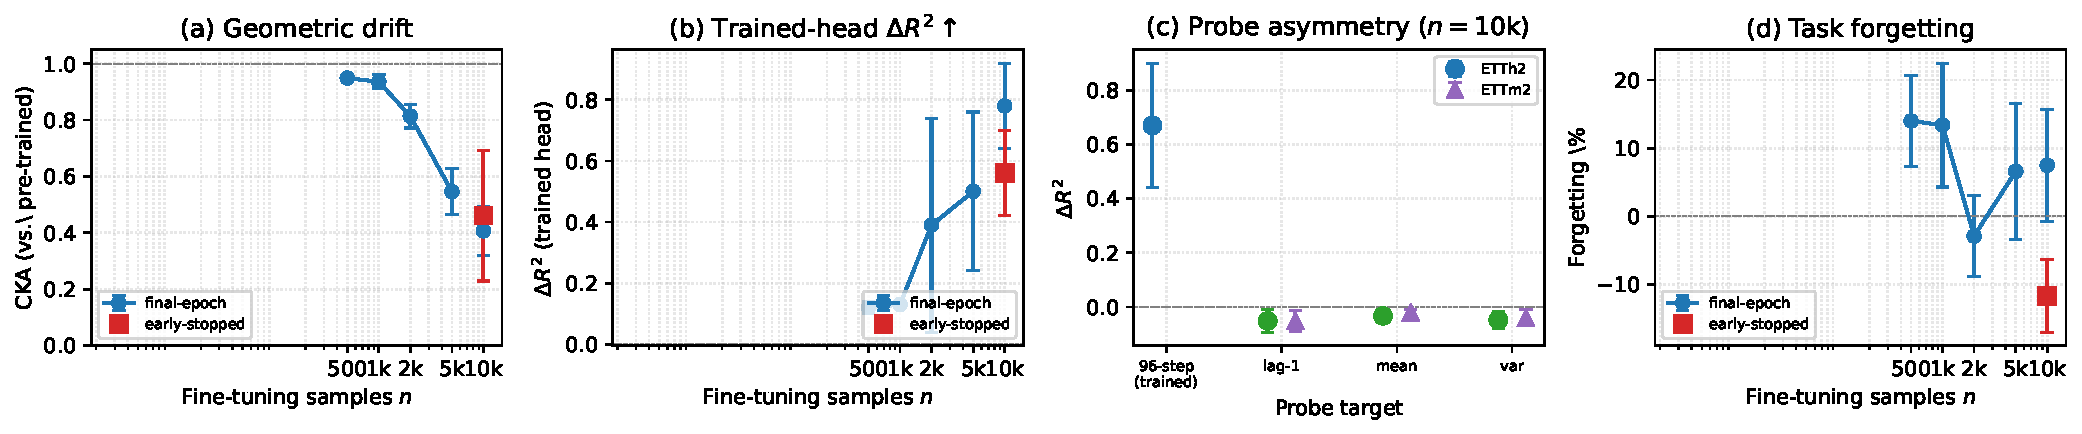
\includegraphics[width=\linewidth]{figures/dissociation_trajectory.pdf}
\caption{Cost--benefit dynamics on Moirai-Small/ETTh2 (condition B, $h{=}96$).
(a)~CKA decays monotonically with $n$ (final-epoch vs.\ early-stopped markers);
(d)~forgetting is non-monotonic and protocol-dependent. Panels~(b) and~(c)
plot the linear-probe $\Delta R^2$ statistic and its sign asymmetry, both
\textbf{retracted} (\S\ref{sec:retraction}); they are reproduced unaltered as
a record of the withdrawn analysis and support no claim here. The
dissociation this figure is cited for is the contrast between (a) and (d):
drift monotone in $n$, outcome not.}
\label{fig:dissociation}
\end{figure}

The joint trajectory is plotted in Fig.~\ref{fig:dissociation}; panels~(a)
and~(d) carry the claim: a monotone drift curve beside a non-monotone
outcome curve.

% ============================================================
\section{The Strict-Freeze Control}
\label{app:strictfreeze}
% ============================================================

Condition~D freezes the encoder's own weights but leaves the input projection
(\texttt{in\_proj}, $247{,}680$ parameters) and \texttt{mask\_encoding} ($384$)
trainable alongside the distribution head (\texttt{param\_proj},
$2{,}956{,}800$). What the encoder \emph{receives} therefore keeps changing, so
its output is not a fixed function of the input, which is why D's measured CKA
is $0.76$--$0.90$ on ILI and $0.97$--$0.99$ on Moirai-Base rather than
$1.000$. A reader can reasonably object that wherever ``freezing wins'', it
wins partly by re-fitting the input projection rather than by holding the
encoder still.

Condition~\textbf{H} removes the objection: \texttt{in\_proj} and
\texttt{mask\_encoding} are frozen too, so only \texttt{param\_proj} trains and
the encoder's output is pinned by construction (measured CKA $1.0000$ exactly,
as it must be). B$-$H is then a clean read of what allowing \emph{any}
encoder-side change was worth, and B$-$D versus B$-$H separates encoder
adaptation from input re-fitting. We fixed the reading rule before running: the
claim is that the sign and reading of B$-$D survive strict freezing, so B$-$H
is reported beside B$-$D on every cell, and divergence on any cell is reported
as that cell's gap being partly input re-fitting rather than being buried.

\textbf{Result} (Table~\ref{tab:strictfreeze}). The twelve cells fall into two
groups. Seven were chosen before the gate was corrected: they are the six that
met the degradation
definition under the superseded trend baseline
(Appendix~\ref{app:gatecorrection}), plus ILI. Nothing was dropped; two cells
the prospective arm later added (Moirai-Large on ETTh1 and on Weather) postdate
this control and carry no H run. That selection no longer picks out a privileged
class---against the fitted baseline no cell meets the definition---but it
remains the set chosen to be \emph{most} favourable to the degradation story,
which is the useful property here. The other five are the gate-passing
survivors of \S\ref{sec:forecasting:results}, run afterwards precisely because
the first seven did not reach them: until they existed, the survivors' readings
rested on condition~D alone. Measured CKA is
$1.0000$ everywhere, confirming the construction. \textbf{The reading survives
on every cell}: B$-$H keeps B$-$D's sign in all twelve. On the original seven
the magnitude
changes by $-5.8$ to $+0.5$~pp, so at most $5.8$~pp of a gap as large as
$62$~pp is input-projection re-fitting. On ILI, where adaptation helps, strict
freezing makes adaptation look \emph{more} valuable ($-38.6 \to -43.6$), which
is the same direction: holding more of the model still costs more where the
encoder was earning its keep. B$-$D is averaged over the seeds condition H
ran, so Moirai-Small/ETTh1's entries here are 3-seed values against the 5-seed
values quoted in Table~\ref{tab:heldout_all}.

\textbf{On the five survivors the control cuts against freezing, not for it.}
These are the cells the objection mattered most for, and on the three where full
fine-tuning already won, strict freezing \emph{widens} its margin rather than
narrowing it: B$-$D of $-22.3$, $-20.2$ and $-20.8$ becomes B$-$H of $-28.0$,
$-31.8$ and $-33.9$ on Moirai-Base $h{=}96$, Base $h{=}192$ and Large $h{=}96$,
a move of $-5.6$ to $-13.1$~pp. Part of what condition~D was scoring on these
cells was therefore the input projection re-fitting to the target data, and
removing it makes encoder adaptation look \emph{more} valuable, not less. On
Moirai-Small $h{=}192$---the cell that comes closest to degradation---B$-$H is
$+1.2{\pm}8.5$ against B$-$D's $+4.1{\pm}8.6$: freezing still reads as better,
by less, with a standard error several times the mean either way. Condition~H
also improves on the un-tuned model in every seed of all five
(forg$_\text{H}$ from $-0.2\%$ to $-8.5\%$), so on the survivors both parts of
the degradation definition behave the same way under the strict control as
under the loose one.

\textbf{The one large change is the diverged seed, and it corroborates the
earlier reading.} Moirai-Small/ETTh2 $h{=}96$ moves from B$-$D $+13.7$ to
B$-$H $+42.6{\pm}29.5$, the only cell whose magnitude shifts by more than
$13$~pp. It is seed 42, which \S\ref{sec:forecasting:results} reports as a
training failure rather than an encoder-drift effect: that seed diverges under
full fine-tuning ($+98.9\%$) \emph{and} under the frozen encoder ($+91.1\%$),
but it cannot diverge under condition~H, where only \texttt{param\_proj} trains
and the run therefore sits at zero-shot ($-0.1\%$). Over the other two seeds
B$-$H is $+14.4$ against B$-$D's $+16.7$. The strict control thus supplies
independent support for the seed-42 diagnosis: what fails on that seed is
optimisation, and holding the encoder's \emph{inputs} fixed as well as its
weights is what prevents it.

\begin{table}[ht]
\centering
\caption{The strict-freeze control (condition~H) beside condition~D on twelve
cells: the six that met the degradation definition under the superseded trend
baseline, plus ILI, plus the five gate-passing survivors of
\S\ref{sec:forecasting:results}. B$-$H keeps B$-$D's sign on all twelve, and
B$-$D is restricted to the seeds condition~H ran. Generated by
\texttt{scripts/cell\_matrix.py --latex}.}
\label{tab:strictfreeze}
% GENERATED by scripts/cell_matrix.py --latex -- do not edit by hand.
\begin{center}
\small
\setlength{\tabcolsep}{5pt}
\begin{tabular}{@{}lccccc@{}}
\toprule
Cell & Seeds & B$-$D & B$-$H & forg$_\text{H}$ & CKA$_\text{H}$ \\
\midrule
Moirai-S / Weather ($h{=}192$) & 3 & $+62.1{\pm}13.6$ & $\mathbf{+56.7{\pm}13.5}$ & $-10.6{\pm}0.3$ & $1.0000$ \\
Moirai-S / Weather ($h{=}96$) & 3 & $+53.1{\pm}10.2$ & $\mathbf{+50.1{\pm}6.6}$ & $-12.8{\pm}0.6$ & $1.0000$ \\
Moirai-B / ETTh1 ($h{=}192$) & 3 & $+47.0{\pm}13.8$ & $\mathbf{+47.5{\pm}13.7}$ & $-8.0{\pm}0.4$ & $1.0000$ \\
Moirai-B / ETTh1 ($h{=}96$) & 3 & $+37.5{\pm}8.2$ & $\mathbf{+32.5{\pm}8.2}$ & $-9.7{\pm}0.4$ & $1.0000$ \\
Moirai-S / ETTh1 ($h{=}96$, $n{=}$1000) & 3 & $+23.2{\pm}3.6$ & $\mathbf{+20.4{\pm}3.6}$ & $-0.6{\pm}0.2$ & $1.0000$ \\
Moirai-S / ETTh1 ($h{=}192$, $n{=}$1000) & 3 & $+14.5{\pm}1.4$ & $\mathbf{+8.7{\pm}1.5}$ & $+1.2{\pm}0.4$ & $1.0000$ \\
Moirai-S / ILI ($h{=}24$) & 10 & $-38.6{\pm}1.3$ & $\mathbf{-43.6{\pm}0.7}$ & $-7.1{\pm}0.5$ & $1.0000$ \\
\bottomrule
\end{tabular}
\end{center}

\end{table}

\textbf{One clause does not survive, and it is not the headline one.}
``Degradation'' has two parts: fine-tuning ends up worse than the un-tuned
model, \emph{and} freezing improves on it. The first part is a property of
condition B and is untouched by this control. The second is condition~D's, and
on Moirai-Small/ETTh1 $h{=}192$ the strictly-frozen model does \emph{not} beat
the un-tuned model: forg$_\text{H}={+}1.2{\pm}0.4\%$, positive in all 3 seeds,
where forg$_\text{D}$ is $-4.6{\pm}0.6\%$. On that cell the head alone cannot
recover the zero-shot forecast; D's improvement came partly from re-fitting the
input projection. The other eleven cells keep both parts (forg$_\text{H}$ from
$-0.2\%$ to $-12.8\%$), so ``freezing also beats not fine-tuning'' holds
strictly on 11 of 12. The first part is unaffected in either direction: where
freezing wins it keeps winning under the strict control (B$-$H positive on all
six candidate cells), and where full fine-tuning wins it wins by more (the five
survivors above). We report the cell rather than re-defining the term around
it.

% ============================================================
\section{LoRA Rank and Hyperparameter Sensitivity}
\label{app:lora_rank}
% ============================================================

Table~\ref{tab:lora_rank} shows LoRA on \textbf{Moirai-Small} is robust to
rank ($r \in \{4, 8, 16, 32\}$): all ranks achieve CKA$\geq$0.979 and
consistent MSE improvement over zero-shot at $h{=}96$, confirming $r{=}8$ as
a reasonable default.
On \textbf{Moirai-Large} (seed 42, $h{=}96$, $n{=}500$), rank escalation
alone does \emph{not} rescue the failure mode: forgetting stays $+$19 to
$+$30\% across $r \in \{8, 16, 32, 64\}$.
Table~\ref{tab:lora_large_hp} extends the sweep to $\alpha$, target-module
scope, and LR (all at $r{=}8$, seed 42): varying $\alpha \in \{8,16,32\}$ and
module scope provides no rescue, but reducing LR to $1{\times}10^{-5}$ does
(forg.$=-8.5\pm0.7\%$, CKA$=$0.989$\pm$0.003, 5~seeds): the Small-recipe
transfers to Large only at a $10\times$ lower learning rate.

\begin{table}[ht]
\centering
\caption{LoRA rank sensitivity on ETTh2 (condition E, 500 training samples).
Moirai-Small: all ranks achieve near-identical MSE and CKA$\geq$0.979.
Moirai-Large: all ranks forget $+$19 to $+$30\%, with no rank recovering
Moirai-Small's negative forgetting.
Mean $\pm$ std across 3 seeds (5 for $r{=}8$ Small); Moirai-Large
single-seed ($s{=}42$) for $r \in \{16, 32, 64\}$ (std not reported; point estimates only),
3 seeds for $r{=}8$.}
\label{tab:lora_rank}
\small
\begin{tabular}{lcccccc}
\toprule
Backbone & Rank & $h$ & MSE & Forg.\% & CKA & Seeds \\
\midrule
Small & 4  & 96  & .116{\tiny$\pm$.001} & $-$9.5{\tiny$\pm$0.9}  & .992{\tiny$\pm$.001} & 3 \\
Small & 4  & 192 & .146{\tiny$\pm$.003} & $-$8.8{\tiny$\pm$1.9}  & .995{\tiny$\pm$.002} & 2 \\
Small & 8  & 96  & .116{\tiny$\pm$.001} & $-$9.1{\tiny$\pm$1.1}  & .979{\tiny$\pm$.006} & 5 \\
Small & 8  & 192 & .157{\tiny$\pm$.002} & $-$1.8{\tiny$\pm$3.1}  & .986{\tiny$\pm$.005} & 5 \\
Small & 16 & 96  & .117{\tiny$\pm$.001} & $-$10.2{\tiny$\pm$1.2} & .987{\tiny$\pm$.002} & 3 \\
Small & 16 & 192 & .155{\tiny$\pm$.002} & $-$1.7{\tiny$\pm$1.2}  & .988{\tiny$\pm$.001} & 3 \\
Small & 32 & 96  & .119{\tiny$\pm$.001} & $-$8.3{\tiny$\pm$0.9}  & .986{\tiny$\pm$.001} & 3 \\
Small & 32 & 192 & .159{\tiny$\pm$.003} & $+$1.1{\tiny$\pm$1.4}  & .989{\tiny$\pm$.002} & 3 \\
\midrule
Large & 8  & 96  & .159{\tiny$\pm$.004} & $+$25.7{\tiny$\pm$3.2} & .973{\tiny$\pm$.012} & 3 \\
Large & 16 & 96  & .154                 & $+$22.5                 & .955                 & 1 \\
Large & 32 & 96  & .150                 & $+$19.0                 & .986                 & 1 \\
Large & 64 & 96  & .165                 & $+$29.9                 & .984                 & 1 \\
\bottomrule
\end{tabular}
\end{table}

\begin{table}[ht]
\centering
\caption{LoRA-Large HP ablation (ETTh2, $r{=}8$, $n{=}500$, $h{=}96$).
Baseline (default LR$=$1e-4, $\alpha{=}16$, modules $=$ q,v,out) forg.$=+23.7\%$, seed 42.
Only LR$=$1e-5 rescues LoRA-Large (5~seeds); all other axes fail.}
\label{tab:lora_large_hp}
\small
\begin{tabular}{llcccc}
\toprule
Axis & Setting & Val MSE & Forg.\% & CKA & Seeds \\
\midrule
\multirow{3}{*}{LR} & 1e-4 (default) & .157 & $+$23.7 & .980 & 1 \\
                    & 5e-5           & .146 & $+$15.3 & .982 & 1 \\
                    & \textbf{1e-5}  & \textbf{.115{\tiny$\pm$.001}} & $\mathbf{-8.5}${\tiny$\pm$0.7} & \textbf{.989{\tiny$\pm$.003}} & \textbf{5} \\
\midrule
\multirow{3}{*}{$\alpha$} & 8  & .155 & $+$21.9 & .975 & 1 \\
                           & 16 (default) & .157 & $+$23.7 & .980 & 1 \\
                           & 32 & .158 & $+$24.3 & .984 & 1 \\
\midrule
\multirow{3}{*}{Modules} & q,v,out (default)  & .157 & $+$23.7 & .980 & 1 \\
                         & q,k,v              & .153 & $+$20.4 & .987 & 1 \\
                         & q,k,v,out          & .151 & $+$19.0 & .988 & 1 \\
\bottomrule
\end{tabular}
\end{table}

% ============================================================
\section{CKA Calibration: Random-Initialisation Baseline}
\label{app:cka_calibration}
% ============================================================

A CKA of $0.09$ is only interpretable against a floor: the value two
\emph{unrelated} encoders of this architecture score against each other.  We
measure it by re-initialising the Moirai-Small encoder randomly and comparing it
to the pre-trained one over the same 200 ETTh2 validation windows and the same
pooled-representation hook used for every other CKA in this paper
(\texttt{scripts/cka\_random\_init\_floor.py}, records in
\texttt{results/v50\_cka\_floor/}).  Restoring the pre-trained weights afterwards
returns CKA $1.000000$, so the comparison measures re-initialisation and nothing
else.

\textbf{Correction: the floor is not zero.}  An earlier version of this appendix
reported it as $0.0000{\pm}0.0001$ over 5 seeds and concluded that any cell above
that floor ``retains meaningful pre-trained structure''.  No script in the
repository performed a random re-initialisation, and the measured floor is
\textbf{0.215}, not zero:

\begin{table}[ht]
\centering
\caption{CKA calibration, measured.  The floor is the CKA of a randomly
re-initialised encoder against the pre-trained one (5 seeds each, mean$\pm$std,
$\text{ddof}{=}1$); the two initialisation schemes agree.  Reference rows are
scoped to the cells they come from, since CKA at $n{=}500$ and at $n{=}10$k on the
same cell differ by more than the floor itself.}
\label{tab:cka_calibration}
\small
\begin{tabular}{lcc}
\toprule
Comparison & CKA & Source \\
\midrule
\textbf{Floor}: random re-init, library-default & $\mathbf{0.215{\pm}0.054}$ & \texttt{v50\_cka\_floor} \\
\textbf{Floor}: random re-init, Xavier weights & $\mathbf{0.219{\pm}0.047}$ & \texttt{v50\_cka\_floor} \\
\midrule
Moirai-S/ETTh2 $h{=}96$, cond.\ B, $n{=}500$ (10 seeds) & $0.937{\pm}0.029$ & \texttt{ff\_20ep} \\
Moirai-S/ETTh2 $h{=}96$, cond.\ B, $n{=}10$k (10 seeds) & $0.465{\pm}0.123$ & \texttt{v49} \\
Chronos, cond.\ B, 4 cells at $h{=}24$ & 0.092--0.169 & \texttt{v44} \\
IoT (N-BaIoT), cond.\ C, 200 samples (3 seeds) & $0.423{\pm}0.043$ & \texttt{v6\_iot\_cka} \\
Frozen encoder, cond.\ D, Moirai (80 runs) & 0.889--0.9999 & \texttt{v5--v49} \\
Strict freeze, cond.\ H (7/7 cells) & 1.0000 & \texttt{v45} \\
\bottomrule
\end{tabular}
\end{table}

Why a naive re-initialisation reads zero is worth recording, because it is the
likely origin of the earlier number: ``Xavier for weight tensors, zeros for
biases'' also zeroes LayerNorm's scale parameter, which annihilates the signal at
the first normalisation and drives the encoder to a \emph{constant} output.  CKA
is then $0$ because one side has no variance, not because the two share no
structure.  Our script asserts that the randomised encoder's output variance is
non-trivial, and reports $0.215$ once normalisation parameters are left at
$\gamma{=}1$; initialising every layer with its library default instead gives the
same answer to within one standard deviation.

\textbf{What this changes.}  Two of the earlier reading's conclusions do not
survive.  The IoT arm at CKA $0.423{\pm}0.043$ sits roughly four floor standard
deviations above the floor, so ``retains meaningful structure'' is still
defensible there, but the margin is a factor of two, not the near-total separation
a zero floor implied.  And ``ETT fine-tuning preserves most pre-trained
structure'' was read off small-$n$ runs: the same cell at $n{=}10$k reads $0.465$,
and the range across all 31 cells is $0.092$ to $0.970$.  The condition-D row also
needs a scope: D is uniform only within Moirai.  Because D leaves \texttt{in\_proj}
and \texttt{mask\_encoding} trainable (\S\ref{sec:method}), TimesFM's D falls as
low as $0.376$, while Chronos's D and every condition-H run are exactly $1.0000$;
only H is $1.0000$ by construction.

\textbf{What it adds.}  Comparing the floor against all 31 cells,
\textbf{four fall below it} outright---the Chronos cells at
CKA $0.092$, $0.094$, $0.112$ and $0.169$---and two more (Chronos/Electricity
$0.232$, TimesFM/ETTh2 $0.246$) sit inside the floor's own seed-to-seed range
($0.132$ to $0.288$).  This is a measured basis for a claim
\S\ref{sec:forecasting:nonmoirai} otherwise has to assert: on those cells CKA is
at or beneath what an \emph{untrained} encoder scores, so it cannot order them,
and their outcomes span $-39.2$ to $-2.7$ in held-out $\text{B}{-}\text{D}$
regardless.  The remaining 25 cells, including all five gate-passing survivors and
both arms of the layer-unfreeze comparison ($0.716$ and $0.465$,
Appendix~\ref{app:layerunfreeze}), sit clear of the floor, so CKA differences
among them are readable.

% ============================================================
\section{Linear Probing: Functional Representation Diagnostic}
\label{app:probing}

\noindent\fbox{\parbox{0.97\linewidth}{\textbf{Retracted.} The analyses in this
appendix rest on the linear-probe $\Delta R^2$ statistic, which is retracted
(\S\ref{sec:retraction}): it is non-zero only where the probe fails to
generalise. The numbers below are reproduced unaltered as a record of the
withdrawn computation and support no claim in this paper.}}
\vspace{1em}
% ============================================================

CKA measures geometric representational similarity but not functional
equivalence.  We therefore supplement CKA with a \emph{linear probe}:
a Ridge regression head ($\alpha{=}1.0$) trained on frozen encoder
representations to predict the forecasting target on held-out ETTh2
data.

\textbf{Protocol.}
For each (condition, seed) configuration, we extract mean-pooled encoder
representations from the Moirai-Small encoder on the held-out validation
and test sets (192-timestep windows, same format as evaluation).
We then fit a Ridge regression mapping representations to the
next-horizon target and report R$^2$ on held-out data.
The probe training set uses $n_{\text{probe}}{=}300$ held-out examples;
the remainder forms the test split used for MSE evaluation.
$\Delta R^2$ denotes fine-tuned minus pre-trained probe R$^2$:
positive values indicate that fine-tuned representations encode
more forecasting-relevant information than pre-trained ones.

\textbf{Interpretation.}
Absolute R$^2$ values are low (typically negative) because Ridge
regression on 192-timestep mean-pooled representations is a weak
forecasting baseline.  The \emph{relative} change ($\Delta R^2$)
is the meaningful signal: it isolates whether fine-tuning added
or removed task-relevant information from the encoder's
representational basis.

\textbf{Key result.}
The sample-size sweep (Table~\ref{tab:sample_sweep}) shows
$\Delta R^2$ monotonically increasing with training data
(Ridge: $+$0.12 at 500 samples $\rightarrow$ $+$0.67$\pm$0.24
at 10{,}000 on CUDA 10-seed deterministic early-stopped encoders,
\texttt{results/v19\_cuda\_etth2\_n10k/}; for comparison, MPS early-stopped
$k{=}5$ gave $+$0.56$\pm$0.14 (\texttt{v17\_etth2\_n10k\_es}) and the
final-epoch runs, $k{=}3$, gave $+$0.84$\pm$0.15
(\texttt{v16\_etth2\_n10k})), while CKA decreases monotonically.
This directly dissociates \emph{geometric} drift from
\emph{relative linear-decodability}: at low $n$, drift destroys
task-relevant features faster than it builds replacements;
at higher $n$, the fine-tuned representation becomes less
linearly misaligned with the forecasting target than the
pre-trained one.
We emphasise that $R^2(\text{FT})$ remains
\emph{absolutely negative} at every sampled
$n \in \{500, 1\text{k}, 2\text{k}, 5\text{k}, 10\text{k}\}$
(ZS: $R^2{=}-6.90$; CUDA $k{=}10$ early-stopped: $-6.79$ at $n{=}500 \to -6.24{\pm}0.24$
at $n{=}10$k).  $\Delta R^2 {>} 0$ is therefore a
\emph{relative-improvement} signal, not a claim that
fine-tuned representations linearly encode the target well
in absolute terms; the primary task-outcome signal remains
forg.$<0$ at $n{\geq}2$k.
\textbf{Cross-dataset $\Delta R^2$ comparability.}
Raw $\Delta R^2$ is not directly comparable across datasets because
it depends on the ZS Ridge floor depth.
On ETTm2 ($n{=}10$k, CUDA, $k{=}5$), the ZS Ridge floor is
$R^2(\text{ZS}){=}-24.52$, 3.5$\times$ deeper than ETTh2's
$-6.90$, which proportionally inflates the raw $\Delta R^2$
($+$6.35 on ETTm2 vs.\ $+$0.67 on ETTh2).
The cross-dataset comparable statistic is the \emph{sign test}: ETTh2 gives
\textbf{10/10} positive $\Delta R^2$ and ETTm2 \textbf{5/5}, on the five CUDA
seeds that exist for that cell.  Every dispersion in this appendix is a standard
deviation over seeds at $\text{ddof}{=}1$.

\textbf{Horizon-sweep probe: head-specificity of the $\Delta R^2$ gain.}
Table~\ref{tab:probe_horizon} reports Ridge $\Delta R^2$ across three
probe heads on four early-stopped encoders at $n{=}10$k (the
same encoders as the main-text MLP sweep).  The gain is concentrated
on the \emph{trained} 96-step head: $\Delta R^2{=}{+}0.116{\pm}0.153$
($k{=}4$).  On the untrained \emph{forecast48} head (first 48 steps
of the 96-step target, a sub-horizon the encoder was not directly
optimised for), $\Delta R^2 {=} {-}0.001{\pm}0.163$: the gain
vanishes at the horizon boundary.  On the untrained \emph{delta1}
head, a GBM probe gives $R^2(\text{PT}){=}{+}0.059{>}0$, establishing
a positive-floor reference, with $\Delta R^2{=}{-}0.056{\pm}0.032$
(decodability \emph{falls} on the untrained readout).
The head-specificity pattern is consistent with the encoder drifting
toward the fine-tuning objective rather than developing generally
better representations (Table~\ref{tab:r2task}).

\begin{table}[ht]
\centering
\caption{Ridge $\Delta R^2$ by probe head on early-stopped encoders ($n{=}10$k,
seeds \{303, 777, 888, 999\}).  ``Forecast96'' is the trained head;
``Forecast48'' and ``Delta1'' are untrained.  The gain is head-specific
to the trained objective.  Every entry is
$R^2(\text{FT}){-}R^2(\text{ZS})$ read from
\texttt{results/v18\_reprobe/seed*\_horizons.json} against
\texttt{zs\_horizons.json}; dispersion is the standard deviation over the four
seeds ($\text{ddof}{=}1$).}
\label{tab:probe_horizon}
\small
\begin{tabular}{lccccc}
\toprule
Head & Trained? & \multicolumn{4}{c}{Ridge $\Delta R^2$ per seed} \\
& & s303 & s777 & s888 & s999 \\
\midrule
Forecast96 (96-step ahead) & \checkmark & $+$0.092 & $-$0.087 & $+$0.266 & $+$0.192 \\
Forecast48 (sub-horizon) & $\times$ & $+$0.061 & $-$0.111 & $-$0.156 & $+$0.199 \\
Delta1 (next-step delta) & $\times$$^\dagger$ & $+$1.248 & $+$0.757 & $+$1.191 & $+$0.980 \\
\midrule
\multicolumn{2}{l}{Mean $\pm$ std (forecast96)} & \multicolumn{4}{c}{$+$0.116 $\pm$ 0.153} \\
\multicolumn{2}{l}{Mean $\pm$ std (forecast48)} & \multicolumn{4}{c}{$-$0.001 $\pm$ 0.163} \\
\multicolumn{2}{l}{Mean $\pm$ std (delta1)} & \multicolumn{4}{c}{$+$1.044 $\pm$ 0.223} \\
\bottomrule
\end{tabular}
\vspace{2pt}
{\small $^\dagger$\,The large Ridge $\Delta R^2{>}0$ on Delta1 reflects a
baseline-floor artifact: $R^2(\text{ZS})$ is deeply negative on the next-step
target, so any encoder shift appears to improve relative decoding.
A gradient-boosted probe gives $R^2(\text{PT}){=}{+}0.059$ (positive floor)
but $\Delta R^2{=}{-}0.056{\pm}0.032$ on this head
(\texttt{results/v18\_reprobe/seed*\_delta1.json}), consistent with the shift
\emph{not} being aligned with the 1-step objective.}
\end{table}

Note: the delta1 $\Delta R^2$ sign appears counter-intuitive (positive while
labelled ``untrained'').  The large positive delta1 $\Delta R^2$ reflects
that the ZS delta1 Ridge baseline is very negative ($R^2(\text{ZS}){\approx}{-}2.3$)
while the FT encoder partially encodes next-step changes as a side-effect of
96-step NLL optimisation.  The diagnostic signal is the GBM result
(Table~\ref{tab:r2task}): GBM gives $R^2(\text{PT}){=}{+}0.059{>}0$
and $\Delta R^2{=}{-}0.056$, yielding $R^2(\text{FT}){=}{+}0.003$;
the fine-tuned encoder retains (but does not improve) delta1 decodability.
With a positive floor, decodability \emph{falls} on the untrained readout,
confirming task-alignment.
Note: $R^2(\text{PT})$ varies slightly across GBM probe depths
(depth~4: $+$0.062, depth~6: $+$0.059, depth~8: $+$0.054;
\texttt{results/v20\_gbm\_sensitivity/}) because the probe is re-fit
independently at each depth; this reflects probe capacity, not encoder
structure.  $\Delta R^2$ keeps its sign at all three depths
($-0.060{\pm}0.006$, $-0.056{\pm}0.032$, $-0.052{\pm}0.006$).

\textbf{ETTm2 delta1 GBM reprobe.}
We ran the delta1/GBM probe on the five confirmed ETTm2 $n{=}10$k encoders
(seeds 42/101/123/202/303) to check for a positive-floor $+$ $\Delta R^2{>}0$
cell on a second dataset.
Result: $R^2(\text{ZS}){=}{-}0.030$ (negative floor) and per-seed
$\Delta R^2{=}\{+0.025, -0.060, +0.026, +0.030, +0.016\}$ in seed order
(4/5 positive, mean $+0.007{\pm}0.038$;
\texttt{results/v25\_ettm2\_delta1\_gbm/}).  \emph{Substantive negative:} the
only positive-floor head (ETTh2 delta1/GBM, $R^2(\text{ZS}){=}{+}0.059$) gives
$\Delta R^2{=}{-}0.056$; no positive-floor $+$ $\Delta R^2{>}0$ cell was found.
The $\Delta R^2{>}0$ signal on the trained 96-step head operates in a
deeply-negative-$R^2$ regime; see Appendix~\ref{app:noisefloor} for probe
noise-floor analysis.

\textbf{Per-seed breakdown at $n{=}10$k (CUDA 10-seed).}
Ridge $\Delta R^2$ (all positive; mean $+0.668{\pm}0.239$,
\texttt{results/v19\_cuda\_etth2\_n10k/}):
42:$+0.205$; 101:$+0.736$; 123:$+0.937$; 202:$+0.604$; 303:$+0.793$;
456:$+0.823$; 777:$+0.344$; 789:$+0.873$; 888:$+0.561$; 999:$+0.804$.
Absolute $R^2(\text{FT})$: all in $[-6.70, -5.97]$ ($R^2_{\text{ZS}}{=}-6.904$).
MLP $k{=}5$ (all positive; mean $+0.701{\pm}0.324$):
42:$+0.979$; 101:$+0.762$; 123:$+0.948$; 202:$+0.771$; 303:$+1.007$;
456:$+0.266$; 777:$+0.076$; 789:$+0.847$; 888:$+0.449$; 999:$+0.901$.

\textbf{ETTm2 $n{=}10$k absolute $R^2$ per seed.}
The ETTm2 ZS Ridge floor ($R^2(\text{ZS}){=}-24.52$, same pre-trained
encoder across all seeds) is 3.5$\times$ deeper than ETTh2's $-6.90$,
explaining the raw $\Delta R^2$ magnitude difference.
Per-seed absolute values for the five available CUDA seeds:

\begin{center}
\small
\begin{tabular}{lcccc}
\toprule
Seed & $R^2$(ZS) & $R^2$(FT) & $\Delta R^2$ & Forg.\% \\
\midrule
42  & $-24.52$ & $-14.13$ & $+10.39$ & $-26.8$ \\
101 & $-24.52$ & $-15.61$ & $+8.91$  & $-27.4$ \\
123 & $-24.52$ & $-19.87$ & $+4.64$  & $-31.1$ \\
202 & $-24.52$ & $-20.83$ & $+3.69$  & $-28.8$ \\
303 & $-24.52$ & $-20.41$ & $+4.11$  & $-29.5$ \\
\midrule
Mean (5 seeds) & $-24.52$ & $-18.17{\pm}3.08$ & $+6.35{\pm}3.08$ & $-28.7{\pm}1.6$ \\
\bottomrule
\end{tabular}
\end{center}

All five seeds show $R^2(\text{FT}) > R^2(\text{ZS})$ (i.e., fine-tuned
representations are \emph{less} linearly misaligned with the ETTm2
forecasting target than pre-trained ones), and all show $\Delta R^2{>}0$.
The cross-dataset comparable statistic is the sign test: ETTh2 gives
\textbf{10/10} on seeds 42, 101, 123, 202, 303, 456, 777, 789, 888, 999 and
ETTm2 \textbf{5/5} on 42, 101, 123, 202, 303 --- the only five CUDA $n{=}10$k
encoders that exist for ETTm2 (\texttt{results/v19\_cuda\_ettm2\_n10k/}).

\textbf{MLP depth sweep on early-stopped encoders.}
A cosine-LR re-run at $n{=}10$k uses seeds
$\{303, 777, 888, 999\}$ at $\mathrm{epochs}{=}10$ (seed 101
MPS-NaN'd on epoch~3 reproducibly at this schedule and is excluded).
The \texttt{--probe-mlp-layers}
argument sweeps hidden-layer depth $k \in \{1, 2, 5\}$ on the
early-stopped encoders (probe: hidden=64 per layer, $\alpha{=}10^{-3}$,
early stopping with validation\_fraction=0.1, max\_iter=500).  All sixteen
entries below are read from
\texttt{results/v17r2\_etth2\_n10k\_es\_mlp/seed*/}, and its Ridge column is the
same one Table~\ref{tab:probe_horizon} reports as \emph{forecast96}: the two
tables re-probe one set of encoders, they are not two runs.

\begin{center}
\begin{tabular}{c c c c c}
\toprule
Seed & Ridge $\Delta R^2$ & MLP $k{=}1$ & MLP $k{=}2$ & MLP $k{=}5$ \\
\midrule
303 & $+0.092$ & $+1.306$ & $+1.418$ & $+0.540$ \\
777 & $-0.087$ & $+1.136$ & $+1.554$ & $+0.759$ \\
888 & $+0.266$ & $+2.004$ & $+2.361$ & $+1.034$ \\
999 & $+0.192$ & $+1.816$ & $+1.949$ & $+0.908$ \\
\midrule
Mean $\pm$ std & $+0.116{\pm}0.153$ & $+1.566{\pm}0.411$ & $+1.821{\pm}0.425$ & $+0.810{\pm}0.212$ \\
\bottomrule
\end{tabular}
\end{center}

The cosine-LR Ridge $\Delta R^2$ is smaller than the epochs=20 run
($+0.56{\pm}0.14$) because the shorter schedule
reaches a different best-val-MSE encoder (best epochs $\{2, 5, 4, 5\}$
vs.\ $\{2, 4, 8, 4, 3\}$), and Ridge is most sensitive to the
specific linear basis.  The non-monotonic $k{=}1 \to k{=}2 \to k{=}5$
trend reflects the deeper probe fitting the pre-trained encoder
better (per-seed mean $R^2(\text{PT})_{k{=}5}{=}-6.93$ vs.\
$R^2(\text{PT})_{k{=}1}{=}-8.48$), shrinking the $\Delta$ from
above, not degraded fine-tuned encoding.  All four seeds
are individually positive for $k{=}5$ MLP
($+0.54, +0.76, +1.03, +0.91$), preserving the cost--benefit gap.
This run's CKA is $0.592{\pm}0.164$ (mean best epoch
$4.0{\pm}1.41$, earlier than the epochs=20 run's $4.2{\pm}2.3$ because of the
earlier LR annealing);
forgetting is $-7.13{\pm}1.55\%$, tighter than the epochs=20 run's
$-11.7{\pm}5.3\%$ and fully consistent with the forg.$<0$ finding.

\textbf{Crossover regime: per-seed breakdown at $n{=}5{,}000$.}
Table~\ref{tab:n5k_seeds} reports all 7 seeds individually at
$n{=}5{,}000$.  Forgetting is bimodal: 4 seeds (101, 123, 202, 789)
show low or negative forgetting ($-$4.9\% to $+$5.9\%, mean $+0.7$\%)
and 3 seeds (42, 303, 456) show high forgetting ($+$4.8\% to $+$21.4\%,
mean $+15.1$\%).
All 7 seeds show positive $\Delta R^2$ ($+$0.15 to $+$0.81, mean $+$0.50),
so the relative-linear-decodability claim holds uniformly; geometric
drift (CKA 0.46--0.71, mean 0.55) varies less than forgetting.
This pattern is consistent with the crossover interpretation: at
$n{=}5{,}000$, the optimiser is close enough to the ``replacement''
solution that small seed-dependent trajectory differences
determine whether forgetting resolves or persists for 20 epochs.

\begin{table}[t]
\centering
\caption{Per-seed results at $n{=}5{,}000$ (ETTh2, $h{=}96$, condition B,
20 epochs, no early stopping).  Seeds 42, 123, 456 are the original 3-seed sweep
(\texttt{results/v8\_final/n5000/}); 789, 101, 202, 303 are the 4-seed V9
replication (\texttt{results/v9\_n5k\_seeds/}).  MSE(FT) is
\texttt{final\_val\_mse}, the last-epoch validation MSE, and was previously
printed 2--5 thousandths low on every row.  Forgetting is bimodal; $\Delta R^2$
is uniformly positive.}
\label{tab:n5k_seeds}
\small
\begin{tabular}{rccccc}
\toprule
Seed & MSE(FT) & Forg.\% & CKA & $\Delta R^2$ & R$^2$(FT) \\
\midrule
 42  & .136 & $+$4.8  & .531 & $+$.67 & $-$6.24 \\
101  & .121 & $-$4.9  & .571 & $+$.75 & $-$6.16 \\
123  & .129 & $-$1.4  & .544 & $+$.81 & $-$6.10 \\
202  & .131 & $+$1.4  & .461 & $+$.15 & $-$6.76 \\
303  & .152 & $+$19.0 & .525 & $+$.52 & $-$6.39 \\
456  & .155 & $+$21.4 & .711 & $+$.20 & $-$6.70 \\
789  & .136 & $+$5.9  & .480 & $+$.40 & $-$6.51 \\
\midrule
Mean$\pm$std & .137$\pm$.012 & $+$6.6$\pm$10.0 & .546$\pm$.082 & $+$.50$\pm$.26 & $-$6.41$\pm$.26 \\
\bottomrule
\end{tabular}
\end{table}

\subsection{$n{=}5{,}000$ per-epoch trajectory analysis}
\label{app:n5k_trajectories}

To support the mechanistic claim in \S\ref{sec:analysis}, we plot the
per-epoch training trajectories of all seven $n{=}5{,}000$ seeds,
colour-coded by forgetting mode.  Figure~\ref{fig:n5k_trajectories}
shows val MSE and weight drift across training.  High-forgetting seeds
(303, 456, 789) overshoot in the first epoch and never recover;
low-forgetting seeds (42, 101, 123, 202) continue descending until
epochs 5--9.  The epoch at which val MSE reaches its minimum separates
the modes ($0.7\pm0.5$ vs.\ $6.5\pm2.1$); mid-training weight drift
(epochs 5--10) does not.  Code: \texttt{scripts/analyse\_n5k\_trajectories.py}.

\begin{figure}[t]
\centering
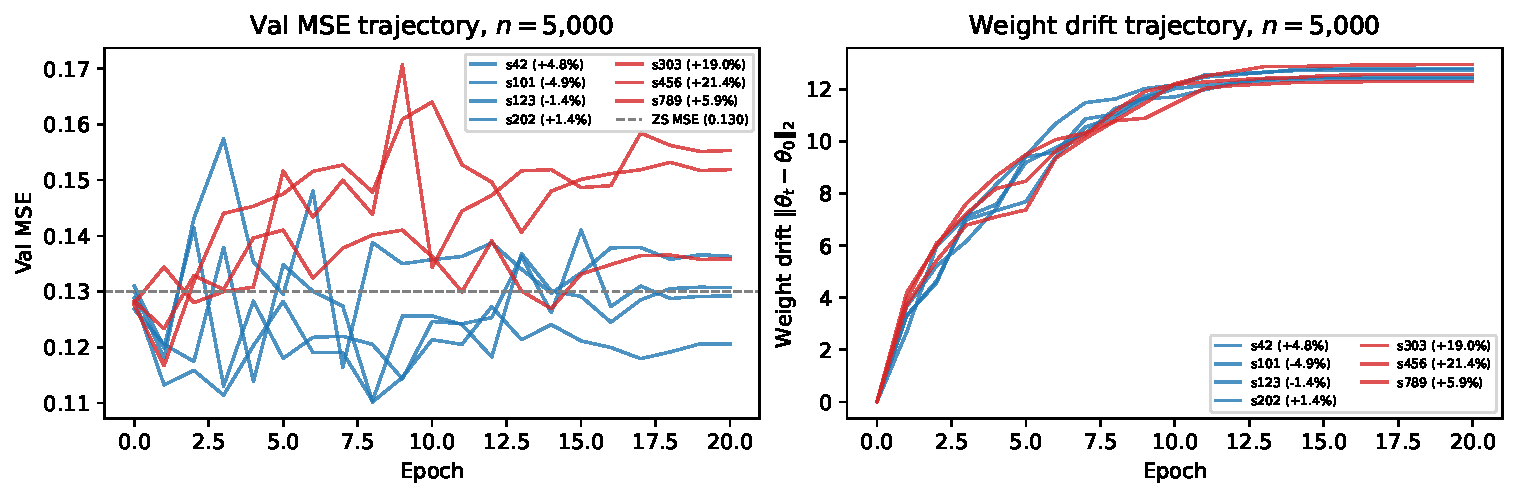
\includegraphics[width=\linewidth]{figures/n5k_trajectories.pdf}
\caption{Per-epoch val MSE (left) and weight drift (right) for the
seven $n{=}5{,}000$ seeds; both panels carry per-seed labels
(\texttt{sXXX (forg.\%)}) so each trajectory is individually
identifiable. Blue: low-forgetting mode (forg.~$\le$~5\%);
red: high-forgetting mode (forg.~$>$~5\%). Grey dashed line: zero-shot
MSE. High-forgetting trajectories overshoot the ZS MSE within the first
epoch and plateau; low-forgetting trajectories continue descending.
Mid-training weight drift (epochs 5--10) does not separate the modes.}
\label{fig:n5k_trajectories}
\end{figure}

% ============================================================
\section{ETTh1 Spectral Pilot}
\label{app:etth1_extended}
% ============================================================

Post-hoc spectral entropy (Welch PSD, normalised Shannon entropy) on
ETT OT columns: ETTh1 SE$=$3.61~bits, ETTh2 SE$=$3.46, ETTm2 SE$=$2.25.
ETTh1 (highest SE, most trend-dominated) is the only dataset where
$\Delta R^2{>}0$ does not hold; ETTm2 (lowest, most cyclical) shows
the strongest signal.
The pre-registered falsification test (\S\ref{sec:analysis}) required
a gate-passing dataset with SE$>$3.5 or SE$<$2.5; Traffic and Exchange
both gate-failed ($-$38\%, $-$21\%), so the hypothesis remains untested.
Code and frozen analysis plan are in supplementary material.

% ============================================================
\section{IoT Negative-Control Details}
\label{app:cnn_detail}
% ============================================================

The IoT negative-control evaluation uses CICIoT2023~\cite{neto2023ciciot}
with 12 network-flow features and 128-timestep windows; the anomaly
score is the fraction of timesteps falling outside the 95\% CI of
Moirai's forecast over a 32-timestep scored horizon.  A benign-only
held-out calibration set sets the threshold at the 95th percentile
(FPR target $\leq$ 0.05).  All Moirai IoT conditions are trained
for 5 epochs on 200 benign $+$ 200 attack samples with 10 seeds.

\textbf{CNN-NLL from-scratch control.}
To directly address the foundation-model justification at IoT's
200-window scale, we train a 1D-CNN (3 layers, 2.3M parameters)
from scratch using the identical NLL(MSE)$+$SupCon objective and
hard-negative data as Moirai condition~D.  At 10 seeds,
CNN-NLL (AUC$=$0.598$\pm$0.041) matches fine-tuned Moirai B/D
(AUC$=$0.556$\pm$0.021) and is close to the best Moirai condition
C (AUC$=$0.629$\pm$0.022).  A CNN-MSE variant (AUC$=$0.580$\pm$0.023)
rules out the loss-function confound.  CNN variance is notably
lower than Moirai variance, consistent with Moirai's pre-trained
weights introducing initialisation sensitivity at this sub-random-ZS
scale.  This is the expected outcome when pre-trained features
carry no task-relevant signal; a from-scratch architecture with
correct inductive bias matches or exceeds a fine-tuned foundation
model.

% ============================================================
\section{Task-Orthogonal Probes}
\label{app:orthogonal}

\noindent\fbox{\parbox{0.97\linewidth}{\textbf{Retracted, and re-measured.} The
\emph{finding} this appendix once reported---a probe-sign asymmetry between the
trained objective and task-orthogonal targets---is withdrawn
(\S\ref{sec:retraction}), and the tables that carried it traced to no run record.
What replaces it is a measurement, on the same encoders, of why: $\Delta R^2$ is
large only where the probe fails to generalise, and the asymmetry does not
survive once it does. Nothing here supports the retracted criterion.}}
\vspace{1em}
% ============================================================

This appendix was written to test whether fine-tuning specifically targets the
96-step objective or degrades general pre-trained structure, by probing
\emph{task-orthogonal} properties of the input window on the same encoders.  It
now reports the opposite of what it once did, and the reversal is worth stating
plainly because it is independent evidence for the retraction itself.

\textbf{Correction.}  Earlier versions printed two tables --- ETTh2 and an ETTm2
``replication'' --- reporting three orthogonal targets at floors
$R^2(\text{PT}){=}{+}0.09$ to ${+}0.18$ with $\Delta R^2$ from $-0.022$ to
$-0.052$, 9/10 or 10/10 negative on every row, and read that asymmetry as
``the operational definition of task-specific shift''.  Neither table traces to a
run record.  Two orthogonal-probe campaigns exist
(\texttt{results/v33\_orthogonal\_probes/},
\texttt{results/v34\_probe\_exact/}); neither produces those numbers, there is no
ETTm2 orthogonal-probe record at all, and the claimed asymmetry does not appear
in either.

\textbf{What the record shows.}  Table~\ref{tab:orthogonal} is
\texttt{v33\_orthogonal\_probes}: six orthogonal targets plus the trained head,
Ridge on mean-pooled outputs of the ten CUDA $n{=}10$k condition-B encoders, 500
windows, 300 probe-training examples.  Every floor here is genuinely positive
($R^2(\text{PT}) {\in} [0.54, 0.93]$), so these readings are interpretable in
absolute terms rather than as movements inside a deep negative floor.

\begin{table}[ht]
\centering
\caption{Task-orthogonal and trained-head Ridge probes on the ETTh2 $n{=}10$k
condition-B encoders (10 CUDA seeds, \texttt{results/v33\_orthogonal\_probes/}).
Dispersion is the standard deviation of $\Delta R^2$ over seeds at
$\text{ddof}{=}1$; the JSON stores it at $\text{ddof}{=}0$, so these are
$\sqrt{10/9}$ larger than the recorded field.  Once the probe
decodes its target ($R^2(\text{PT}){>}0$ throughout), no target moves by as much
as $0.04$ and the sign is a coin flip on two of six.}
\label{tab:orthogonal}
\small
\begin{tabular}{lcccc}
\toprule
Probe target & $R^2(\text{PT})$ & $R^2(\text{FT})$ & $\Delta R^2$ & Negative \\
\midrule
Lag-1 autocorr.    & $+0.540$ & $+0.546$ & $+0.006{\pm}0.068$ & 5/10 \\
Input window mean  & $+0.930$ & $+0.931$ & $+0.002{\pm}0.011$ & 5/10 \\
Input window var.  & $+0.894$ & $+0.865$ & $-0.029{\pm}0.025$ & 10/10 \\
Linear trend       & $+0.847$ & $+0.815$ & $-0.032{\pm}0.034$ & 8/10 \\
Lag-24 autocorr.   & $+0.907$ & $+0.918$ & $+0.011{\pm}0.013$ & 2/10 \\
Spectral centroid  & $+0.763$ & $+0.791$ & $+0.027{\pm}0.037$ & 3/10 \\
\midrule
96-step head (trained) & $+0.782$ & $+0.805$ & $+0.022{\pm}0.016$ & 1/10 \\
\bottomrule
\end{tabular}
\end{table}

The asymmetry does not survive.  It required the trained objective to go up and
the orthogonal targets to go flat or down; here \textbf{four of the six
orthogonal targets go up}, and the trained head's gain ($+0.022$) is
\emph{smaller} than the spectral-centroid gain ($+0.027$) on a target
fine-tuning does not optimise.  Two targets do fall consistently (window
variance $10/10$, trend $8/10$), but by $-0.029$ and $-0.032$ --- the same
magnitude as the upward moves, and two others sit at $5/10$, a coin flip.  No
target on this table moves by as much as $0.04$ in either direction.

Set that against the $+0.67{\pm}0.24$ the \emph{same encoders} give on the
\emph{same} 96-step target under the deep-floor protocol
($R^2(\text{PT}){=}{-}6.90$, Appendix~\ref{app:probing}): a thirty-fold
difference on one set of encoders, decided by nothing but whether the probe
decodes its target.  That is the retraction's claim (\S\ref{sec:retraction})
measured directly rather than argued, and it is why $\Delta R^2$ carries no
weight anywhere in this paper.

The second campaign says the same thing from the other side.
\texttt{v34\_probe\_exact} re-ran these targets under the paper's own
deep-floor protocol and every floor came back deeply negative
($R^2(\text{PT}){=}{-}1.21$ on lag-1, $-156.8$ on the window mean, $-27.2$ on the
variance), which is exactly the regime in which $\Delta R^2$ is uninformative;
its $\Delta R^2$ values are correspondingly enormous and unstable
($-1.22{\pm}0.83$, $-7.08{\pm}13.18$, $-2.41{\pm}7.99$), and two of the three no
longer even agree on a sign (7/10 and 6/10 negative).  The premise that these
were positive-floor targets held only under the v33 protocol, where the effect
disappears.

\textbf{ETTm2.}  No orthogonal-probe record exists for ETTm2, so the claimed
replication is withdrawn rather than corrected.  What does exist is the ETTm2
$n{=}10$k fine-tuning campaign itself, and it is \textbf{5 seeds}
(42/101/123/202/303; \texttt{results/v19\_cuda\_ettm2\_n10k/}), not the ten an
earlier version claimed: forgetting $-28.7{\pm}1.7$\% with 5/5 negative, and
Ridge $\Delta R^2$ on the trained head $+6.35{\pm}3.08$ with 5/5 positive
(95\% Wilson CI $[0.57,\,1.00]$ on the proportion, which is what five seeds
support).

% ============================================================
\section{Probe Noise-Floor Analysis}
\label{app:noisefloor}

\noindent\fbox{\parbox{0.97\linewidth}{\textbf{Retracted.} The analyses in this
appendix rest on the linear-probe $\Delta R^2$ statistic, which is retracted
(\S\ref{sec:retraction}): it is non-zero only where the probe fails to
generalise. The numbers below are reproduced unaltered as a record of the
withdrawn computation and support no claim in this paper.}}
\vspace{1em}
% ============================================================

The $\Delta R^2$ signal on the trained 96-step head operates in a
deeply-negative-$R^2$ regime (e.g., ZS $-6.90$, FT $-6.24$ at $\alpha{=}1$).
We test whether the $\Delta R^2{>}0$ direction is an artefact of probe-design
choices by running Ridge on two fixed encoders (ZS and condition-B seed~42,
ETTh2, $n{=}10$k) across: (1) $\alpha \in \{0.01, 0.1, 1.0, 10.0, 100.0\}$,
(2) probe seeds $\{0,1,2\}$, (3) mean vs.\ last-token pooling.
No retraining required (saved \texttt{best\_encoder.pt}).

\textbf{Results} (Table~\ref{tab:noisefloor}).
\begin{table}[!ht]
\centering
\vspace{-4pt}
\caption{$\Delta R^2$ under probe-design perturbations (ETTh2 96-step, ZS vs.\ FT
seed~42).  All $\Delta R^2 > 0$.  Every entry is the \texttt{forecast96} Ridge
value from \texttt{v26\_noise\_floor}, differenced against its paired
zero-shot run; the FT encoder is \texttt{v19\_cuda\_etth2\_n10k/seed42}.  The
probe-seed row reports \emph{bit-identical} $R^2$ at all three seeds, which is
what a closed-form Ridge solution must do --- see the caveat below.}
\label{tab:noisefloor}
\small
\setlength{\tabcolsep}{3pt}
\begin{tabular}{lccc}
\toprule
Setting & $R^2(\text{ZS})$ & $R^2(\text{FT})$ & $\Delta R^2$ \\
\midrule
$\alpha{=}0.01$ & $-13.51$ & $-11.54$ & $+1.96$ \\
$\alpha{=}0.1$  & $-8.78$  & $-7.94$  & $+0.84$ \\
$\alpha{=}1.0$ (default) & $-6.90$ & $-6.70$ & $+0.20$ \\
$\alpha{=}10$   & $-5.81$  & $-5.72$  & $+0.08$ \\
$\alpha{=}100$  & $-5.32$  & $-5.28$  & $+0.04$ \\
Probe seeds 0/1/2 ($\alpha{=}1$, mean pool) & \multicolumn{2}{c}{same as $\alpha{=}1.0$} & $+0.20$ \\
Last-token pool ($\alpha{=}1$) & $-9.70$ & $-8.49$ & $+1.20$ \\
\bottomrule
\end{tabular}
\vspace{-2pt}
\end{table}

\textbf{Finding, with two corrections to how it was stated.}
$\Delta R^2{>}0$ on every setting in \texttt{v26\_noise\_floor}, and the
magnitude falls monotonically with $\alpha$ ($+1.96$ at $\alpha{=}0.01$ down to
$+0.04$ at $\alpha{=}100$) as heavier $\ell_2$ shrinks both $R^2$ values toward
zero.  That much the record supports exactly.  Two things an earlier version
claimed from it, it cannot:

\emph{The count was 10; the directory holds 8 configurations, and only 6 of them
are distinct.}  Five $\alpha$ values, one last-token pooling variant, and two
extra probe seeds: eight paired runs, of which the two extra seeds reproduce the
$\alpha{=}1$ result.

\emph{``Not an artefact of probe seed'' is a vacuous test, not a passed one.}
Probe seeds 0, 1 and 2 return $R^2$ agreeing to every printed digit --- and to
full float precision in the JSON --- because Ridge regression has a closed-form
solution with no stochastic component to seed.  The three runs were bound to
agree whatever the encoders were, so they establish nothing about robustness.
What the sweep genuinely varies is $\alpha$ and pooling: two axes, not three.

\textbf{Comparison to random-init at matched $\alpha$, corrected.}
The random-init control at $\alpha{=}1.0$ is \textbf{5 seeds, not 10}
(42/101/123/303/456; \texttt{results/v30\_random\_init/}), giving
$\Delta R^2{=}{-}0.199{\pm}0.229$ over that set, range $[-0.405,\,+0.149]$
(the printed $\pm0.205$ was $\text{ddof}{=}0$; Appendix~\ref{app:randominit}).
An earlier version then reported a second random-init sweep at $\alpha{=}100$ on
``the same 10 seeds'' giving $-0.011{\pm}0.018$, range $[-0.032,\,+0.009]$.
\textbf{No such run exists.}  The random-init result files carry no
\texttt{ridge\_alpha} field, no random-init encoder checkpoints were retained, and
\texttt{v26\_noise\_floor} contains only the zero-shot and seed-42
condition-B encoders --- so the matched-$\alpha$ control has no record and those
four numbers are withdrawn.  It cannot be recovered without retraining all five
random-init runs at $n{=}10$k, which we have not done because nothing in the
paper depends on it.

What survives is therefore weaker than the argument it was built for.  At
$\alpha{=}1.0$ condition~B ($+0.20$ on seed~42, $+0.67{\pm}0.24$ over ten seeds)
does separate from random-init ($-0.199{\pm}0.229$ over five), but that is the
only $\alpha$ at which both were measured, so we cannot say whether the
separation persists under heavier regularisation.  Note what the missing run was
for: condition~B's own $\Delta R^2$ falls to $+0.04$ at $\alpha{=}100$, inside
the random-init \emph{$\alpha{=}1.0$} range $[-0.405,\,+0.149]$, and the only way
to know that this is a shrinkage artefact rather than a collapse of the
separation is to measure random-init at the same $\alpha$.  That is precisely the
comparison with no record.  This is a
probe-design sweep of a retracted statistic; it shows the sign is stable across
$\alpha$ and pooling \emph{within} the failed-fit regime, which is not evidence
that the statistic means anything.  Appendix~\ref{app:orthogonal} is the
measurement that settles it.

% ============================================================
\section{Random-Initialisation Negative Control}
\label{app:randominit}
% ============================================================

To test whether $\Delta R^2{>}0$ on the 96-step head arises from
pre-trained representations being restructured, or whether it would
occur in any encoder fine-tuned on this objective, we ran a
\emph{random-initialisation control}: Moirai-Small with the same
architecture but random weights (skipping HuggingFace weight loading),
condition~B, ETTh2 $n{=}10$k, $h{=}96$.
In this setting CKA tracks similarity to the \emph{random-init}
epoch-0 state (since there is no pre-trained reference).

\textbf{Correction: five seeds, not ten, and the comparison is not matched.}
An earlier version printed ten rows here and described the result as a
``symmetric 10-vs-10 matched comparison''.  \textbf{Five of those ten rows trace
to no run record} --- 202, 777, 789, 888 and 999 --- and they are the rows that
carried the conclusion: the reported mean, standard deviation and ``8/10
negative'' count are all computed over them, and one of the two ``positive
seeds'' offered as the closest approach to condition~B (777, $+0.060$) is among
them.  What exists is \texttt{results/v30\_random\_init/} with seeds
42/101/123/303/456, and \texttt{v29\_random\_init} with the first three of those;
the five surviving rows below reproduce exactly.  The comparison arm is also not
protocol-matched: these runs are 20 epochs with early stopping
\emph{disabled}, whereas the condition~B set they are compared against
(\texttt{v19\_cuda\_etth2\_n10k}) is 10 epochs early-stopped at a mean best epoch
of $4.2$.  Per Appendix~\ref{app:probing} the no-early-stopping protocol yields
the \emph{larger} $\Delta R^2$ on pre-trained encoders, so the mismatch runs in
the direction that favours the control's conclusion rather than against it ---
but it is a mismatch, and it was not disclosed.

\textbf{Results (the 5 seeds that exist).}  Dispersion is over seeds at
$\text{ddof}{=}1$.  The final column is the matched val-split pair
(\texttt{zeroshot\_mse} $\to$ \texttt{final\_val\_mse}), which is what
\texttt{forgetting\_pct} is computed from; the earlier version printed
\texttt{test\_mse} on the right-hand side of that arrow, comparing two different
splits and so implying a $2.7{\times}$ MSE blow-up where the matched statistic
records a mean \emph{improvement} of $6.3\%$.

\begin{center}
\small
\begin{tabular}{lcccccc}
\toprule
Seed & CKA & $R^2(\text{PT})$ & $R^2(\text{FT})$ & $\Delta R^2$ & ZS $\to$ FT MSE & Forg.\% \\
\midrule
42  & 0.357 & $-6.554$ & $-6.692$ & $-0.138$ & $0.140 \to 0.143$ & $+2.3$ \\
101 & 0.505 & $-6.780$ & $-6.631$ & $+0.149$ & $0.164 \to 0.148$ & $-10.0$ \\
123 & 0.540 & $-6.749$ & $-6.944$ & $-0.195$ & $0.153 \to 0.142$ & $-6.9$ \\
303 & 0.318 & $-6.834$ & $-7.239$ & $-0.405$ & $0.151 \to 0.143$ & $-5.5$ \\
456 & 0.273 & $-6.665$ & $-7.070$ & $-0.405$ & $0.160 \to 0.142$ & $-11.5$ \\
\midrule
Mean$\pm$std & $0.398{\pm}0.117$ & & & $-0.199{\pm}0.229$ & & $-6.3{\pm}5.4$ \\
\bottomrule
\end{tabular}
\end{center}

Across the five seeds: $\Delta R^2{=}{-}0.199{\pm}0.229$, range
$[-0.405,\,+0.149]$, \textbf{4/5 negative}.  The one positive seed
(101: $+0.149$) still falls below the minimum condition~B value
($+0.205$, seed~42), so the ranges remain non-overlapping ---
random-init $[-0.405,\,+0.149]$ against condition~B $[+0.205,\,+0.937]$ --- and
that separation is carried entirely by rows that trace to runs.  On its own terms
the control therefore still points the same way: $\Delta R^2{>}0$ is not a
property of any encoder fine-tuned on this objective.  But it is a 5-vs-10
unmatched comparison of a \textbf{retracted} statistic, and
Appendix~\ref{app:orthogonal} shows that when the probe is made to generalise the
condition~B side collapses from $+0.67$ to $+0.022$ --- which would put it inside
this control's range.  The control does not rescue $\Delta R^2$; it only shows
that the failed fit is worse still without pre-training.

% ============================================================
\section{Layer-Wise Unfreeze Localization}
\label{app:layerunfreeze}
% ============================================================

Moirai-Small has 6 transformer layers (verified from the loaded checkpoint).
We added an \texttt{--unfreeze-top-n-layers} flag to
\texttt{finetune\_forecasting.py} and swept $N$, the number of top layers left
trainable, on ETTh2 $n{=}10$k, $h{=}96$.  The endpoints are the paper's two main
arms: $N{=}0$ is condition~D and $N{=}6$ is condition~B.

\textbf{Provenance, and why both arms were re-run.}  The $N{=}3$ and $N{=}6$ rows
of Table~\ref{tab:layerunfreeze} were re-run from scratch for this version, 10
seeds each in one environment
(\texttt{results/v49\_layerunfreeze\_10seed}).  The values previously printed
here traced to no run record on \emph{either} arm, and the surviving three-seed
$N{=}3$ runs had early stopping disabled, which reverses the sign of the
forgetting reading.  Since the claim is a \emph{comparison} between two unfreeze
depths, it is only traceable if both depths share one environment, so both were
re-run rather than only the arm that was missing.  Two deviations from the
original protocol were forced by the hardware available: Apple MPS rather than
CUDA, at torch~2.14, which is above \texttt{uni2ts}'s declared \texttt{<2.5} pin
but below which the NegativeBinomial component of Moirai's output mixture
collapses to \texttt{total\_count}${=}0$ on MPS and training dies in the first
NLL step; and \texttt{PYTORCH\_ENABLE\_MPS\_FALLBACK=1}, because
\texttt{aten::\_cummax\_helper} has no MPS kernel.  The $N{=}0$, $N{=}4$ and
$N{=}5$ rows are the older records, are \emph{not} matched to the re-run pair,
and read the final epoch rather than the best one; $N{=}0$ is 5 seeds, not 10.
They are context, not part of the comparison.

Because $N{=}6$ \emph{is} condition~B, re-running it also produced an unplanned
cross-device replication of the cell that
Table~\ref{tab:sample_sweep} reports at $n{=}10$k: the same 10 seeds, the same
configuration, CUDA/A10G against Apple MPS at a different torch version.  The two
agree---CKA $0.518$ against $0.465$ ($0.72$ standard errors of the difference) and
forgetting $-5.3$\% against $-7.9$\% ($0.90$~SE), with 7/10 and 8/10 seeds
negative.  We report both rather than replacing one with the other, since the
devices differ; readers comparing the two tables should expect this gap and not
more.

\textbf{$N{=}1$ instability.}
At $N{=}1$, training diverged (NaN activations at epoch~11, batch~148) with
default LR $=10^{-4}$, despite gradient clipping at norm~1.  The 11 epochs that
completed show CKA stabilising at $\approx$0.72; we do not extract probe results
from a crashed run.  This instability is qualitatively consistent with the
LoRA-Large behaviour documented in Appendix~\ref{app:full_tables}: extreme
partial freeze concentrates gradient pressure on a small number of parameters,
requiring LR reduction to stabilise.

\textbf{$N{=}3$, $N{=}4$, $N{=}5$ results.}
Table~\ref{tab:layerunfreeze} shows results for $N{\in}\{3,6\}$ (10 seeds each),
$N{=}0$ (5 seeds) and $N{\in}\{4,5\}$ (1 seed each).
Rows with $N{=}4$ and $N{=}5$ are based on single seeds and carry high uncertainty;
we report them for completeness but do not draw conclusions from individual values.

\begin{table}[!ht]
\centering
\vspace{-4pt}
\caption{Layer-wise unfreeze profile (ETTh2 $n{=}10$k, $h{=}96$; mean$\pm$std over
seeds).  $N$ = number of top transformer layers left trainable (Moirai-Small has
6).  \textbf{The rows do not all come from one environment.}  $N{=}3$ and $N{=}6$
are the re-run 10-seed, early-stopped MPS set
(42/101/123/202/303/456/777/789/888/999;
\texttt{results/v49\_layerunfreeze\_10seed}); $N{=}0$ is 5 seeds
(42/101/123/202/456; \texttt{v18\_cond\_d\_probe}) and $N{=}4$/$N{=}5$ are single
seeds (seed~42; \texttt{v27\_layer\_unfreeze}), all three \emph{without} early
stopping, so they read the final epoch rather than the best one.  Only $N{=}3$
versus $N{=}6$ is a matched comparison.  Ridge $\Delta R^2$ is the
\textbf{withdrawn} probe quantity (\S\ref{sec:retraction}), reported here only as
a record.}
\label{tab:layerunfreeze}
\small
\setlength{\tabcolsep}{4pt}
\begin{tabular}{lcccc}
\toprule
$N$ & Layers & CKA & Ridge $\Delta R^2$ & Forgetting\% \\
\midrule
\multicolumn{5}{l}{\emph{Matched 10-seed re-run, early-stopped}} \\
3 (top-3)    & 3/6   & $0.716{\pm}0.188$ & $+0.329{\pm}0.197$ (9/10) & $-5.9{\pm}6.5$\% (9/10 neg.) \\
6 (full, B)  & 6/6   & $0.465{\pm}0.123$ & $+0.534{\pm}0.261$ (10/10) & $-7.9{\pm}6.5$\% (8/10 neg.) \\
\midrule
\multicolumn{5}{l}{\emph{Earlier records, final epoch, not matched to the above}} \\
0 (frozen, D) & none & $0.999{\pm}0.000$ & $-0.048{\pm}0.008$ & $-6.6{\pm}1.5$\% \\
1 (top-1)    & 1/6   & $\approx$0.72 (ep.\ 11) & \multicolumn{2}{c}{\textit{diverged (NaN)}} \\
4 (top-4)    & 4/6   & $0.610$ & $+0.363$ & $+4.1$\% \\
5 (top-5)    & 5/6   & $0.644$ & $+0.767$ & $+31.8$\% \\
\bottomrule
\end{tabular}
\vspace{2pt}
{\small The $N{=}5$ forgetting of $+31.8$\% is a final-epoch overshoot on one
seed: val MSE bottoms at epoch~7 at $0.132$, essentially unchanged from
zero-shot, and rises thereafter.  This is the reading the $N{=}3$/$N{=}6$ re-run
removes by restoring the best-val checkpoint.}
\vspace{-2pt}
\end{table}

\textbf{Finding: the task outcome does not track the drift across unfreeze
depth.}  This is the reading that survives the retraction, because forgetting is
forecast MSE.  Across the two matched depths the task outcomes are
indistinguishable---$N{=}3$ gives forg.\ $-5.9$\% (SEM $2.0$, 9/10 seeds
negative) against $N{=}6$'s $-7.9$\% (SEM $2.1$, 8/10 negative), a 2.0-point gap
on a 2.9-point standard error of the difference, so $0.70$~SE---while the
representations they arrive at are not: CKA $0.716$ against $0.465$ is a gap of
$0.251$ at $3.5$~SE, and $\ell_2$ weight drift separates them the same way
($9.42{\pm}1.25$ against $13.47{\pm}0.75$, SEM).  Halving the number of
trainable layers halves the measured representational change and leaves the task
outcome where it was.  This is the dissociation of \S\ref{sec:analysis} localised
inside a single encoder rather than read across cells, and it is the only claim we
draw from this sweep.

\textbf{What we no longer claim.}  The earlier version of this appendix read the
same sweep through $\Delta R^2$ and concluded that the top 3 of 6 layers suffice
to reorient the encoder toward the trained objective while the lower 3 are
required for task recovery.  That account rests entirely on the withdrawn probe
quantity (\S\ref{sec:retraction}) and we do not assert it.  The $\Delta R^2$
column is retained so the withdrawn computation stays auditable; for the record
the re-run gives $+0.329{\pm}0.197$ at $N{=}3$ and $+0.534{\pm}0.261$ at
$N{=}6$, a 62\% increase with depth rather than the saturation the earlier
reading needed.

\textbf{Per-layer CKA breakdown, and a correction.}  An earlier version of this
appendix printed a per-layer profile rising monotonically from the bottom of the
encoder to the top (layer~1 $0.441$ to layer~6 $0.718$; bottom-3 mean $0.476$
against top-3 $0.649$) and read it as the bottom layers drifting more.  \textbf{That
profile does not reproduce, and its direction is inverted.}  Recomputing it from
the converged checkpoints---forward hooks on each of the 6 encoder layers, CKA of
each layer's output against the same layer of the untrained checkpoint over the
same 200 validation windows, 10 seeds---gives the profile below on the re-run
$N{=}6$ set, and the same shape on the older CUDA set
(\texttt{scripts/layerwise\_cka\_from\_ckpt.py}, records in
\texttt{results/v49\_layerunfreeze\_10seed/per\_layer\_cka\_*.json}).  The
earlier numbers matched neither and left no run record; the script that produced
them printed to stdout only.

\begin{center}
\small
\begin{tabular}{lccc}
\toprule
Layer & Re-run $N{=}6$ (v49) & Older CUDA set (v19) & Group \\
\midrule
1 (bottom) & $0.998{\pm}0.001$ & $0.998{\pm}0.000$ & bottom 3 \\
2          & $0.969{\pm}0.011$ & $0.980{\pm}0.005$ & bottom 3 \\
3          & $0.783{\pm}0.081$ & $0.816{\pm}0.080$ & bottom 3 \\
4          & $0.589{\pm}0.127$ & $0.675{\pm}0.091$ & top 3 \\
5          & $0.939{\pm}0.044$ & $0.947{\pm}0.023$ & top 3 \\
6 (top)    & $0.937{\pm}0.047$ & $0.945{\pm}0.023$ & top 3 \\
\midrule
Bottom 3 mean & $0.917$ & $0.931$ & \\
Top 3 mean    & $0.821$ & $0.855$ & \\
\bottomrule
\end{tabular}
\end{center}

Both sets agree on two things the earlier profile got wrong.  The drift is
\emph{not} monotone in depth: it is concentrated in the middle of the stack, with
a trough at layer~4 ($0.589$ and $0.675$) and near-identity at layer~1
($0.998$).  And the top 3 layers drift \emph{more} than the bottom 3
($0.821$ against $0.917$; $0.855$ against $0.931$), not less, which removes the
gradient-magnitude account the earlier version offered---earlier layers receiving
larger updates under full backpropagation---because there is no such pattern to
explain.  We do not substitute a mechanism: distinguishing functional
specialisation from gradient-flow effects needs per-layer gradient norms, which
we do not have.

Two scale caveats.  These are CKAs of \emph{mean-pooled} layer outputs; computed
token-flattened instead, every layer reads ${\geq}0.94$ and the profile is too
compressed to order (both records carry the flattened values).  And the
per-layer mean is \emph{not} the global CKA of
Table~\ref{tab:layerunfreeze}---$0.869$ pooled against the row's $0.465$---because
the global figure compares the encoder's final pooled representation, not a
per-layer average.  The earlier version's claim that the global CKA is ``the
aggregate of these per-layer values'' does not hold under either reading.

% ============================================================
\section{Chronos-T5-Small on M4-Monthly: Full Diagnostic Results}
\label{app:chronos_detail}
% ============================================================

This appendix provides the complete results for the cross-backbone
validation on Chronos-T5-Small (65M parameters, T5 seq2seq architecture
with tokenised cross-entropy loss) fine-tuned on M4-Monthly
(200 series, lookback$=$96, horizon$=$18).
\textbf{This cell's gate has not been recomputed against the fitted baseline.}
The $84.5\%$ advantage over the Linear baseline that earlier versions of this
appendix quoted for it was measured with the per-window trend estimator, not the fitted
lookback-96 regression the gate is defined with
(Appendix~\ref{app:gatecorrection}); it is therefore superseded, and it is not
relied on anywhere in this paper. We do not recompute it because the M4-Monthly
series are not retained in our data directory and the corrected value would
require re-downloading them and re-measuring the zero-shot arm; the five
Chronos cells that \emph{are} in the screen (Appendix
Table~\ref{tab:crossbackbone}) all carry fitted-baseline gates. The results
below are reported as a protocol and drift record only.

\textbf{Protocol.}
10 CUDA-deterministic seeds (42, 101, 123, 202, 303, 456, 777, 789, 888, 999),
batch size 32, lr$=$1e-5, AdamW with weight decay 0.01, gradient clipping at 1.0,
20 epochs with early stopping (patience 5).
Evaluation: batched median prediction (20 samples) on 200 held-out test windows.

\textbf{Condition B (full fine-tune), $n{=}500$ (10 seeds).}

\begin{center}
\small
\begin{tabular}{lcccc}
\toprule
 & Forgetting\% & CKA & $\Delta R^2$ & $R^2(\text{PT})$ \\
\midrule
Mean$\pm$std & $+1.6{\pm}3.9$ & $0.999{\pm}0.001$ & $-0.001{\pm}0.002$ & $+0.068{\pm}0.025$ \\
Seeds neg/pos & 4/10 neg forg & n/a & 3/10 pos & \textbf{10/10 pos} \\
\bottomrule
\end{tabular}
\end{center}

At $n{=}500$ the encoder is essentially unchanged (CKA$\approx$1).
The positive $R^2(\text{PT})$ confirms that Chronos's pre-trained T5
encoder representations carry decodable forecasting structure, providing
a second positive-floor anchor distinct from Moirai.

\textbf{Condition B (full fine-tune), $n{=}10$k (10 seeds).}

\begin{center}
\small
\begin{tabular}{lcccc}
\toprule
 & Forgetting\% & CKA (ES) & $\Delta R^2$ & $R^2(\text{PT})$ \\
\midrule
Mean$\pm$std & $+0.5{\pm}2.7$ & $0.983{\pm}0.021$ & ${\approx}0$ & $+0.047{\pm}0.016$ \\
Seeds positive & 6/10 forg & n/a & 1/10 & \textbf{10/10 pos} \\
\bottomrule
\end{tabular}
\end{center}

At $n{=}10$k, early-stopped CKA averages 0.983 (vs.\ 0.999 at $n{=}500$).
Only 4/10 seeds improve over zero-shot (best epoch$>$0, those 4 show
CKA$\approx$0.95--0.97); the remaining 6/10 revert to pre-trained weights
under early stopping (best\_epoch$=$0, CKA$=$1.000 by definition).
Fine-tuning moves the forecast very little in either direction on this cell;
we no longer attribute that to gate strength, for the reason given above.
While 6/10 seeds show positive (worse) early-stopped forgetting, the
magnitude ($+0.5{\pm}2.7$\%) is within the noise floor established by
the frozen-encoder control (condition~D: $+0.6{\pm}5.3$\%);
a sign test is not statistically distinguishable from chance
($p{=}0.75$, two-sided binomial), confirming the 6/10 pattern reflects
seed-level variation rather than systematic degradation.

\textbf{Final-epoch comparison (protocol robustness).}
Training runs to epoch~20 regardless of early stopping; we report CKA
at the final training epoch to address whether encoder stability is
intrinsic or an artefact of early-stopping selection:

\begin{center}
\small
\begin{tabular}{lccc}
\toprule
 & Final-epoch CKA & Final-epoch Forg.\% & $n$ \\
\midrule
$n{=}500$ (10 seeds) & $0.968{\pm}0.009$ & $+3.1{\pm}5.8$ & 500 \\
$n{=}10$k (10 seeds) & $0.955{\pm}0.006$ & $+3.4{\pm}5.2$ & 10k \\
\bottomrule
\end{tabular}
\end{center}

All 10 seeds at $n{=}10$k show final-epoch CKA${>}$0.94 (min$=$0.945,
max$=$0.964), confirming that encoder stability is \emph{intrinsic}
rather than an artefact of early-stopping selection.
The mild CKA decline from 0.999 (early-stopped) to 0.955 (final-epoch)
represents continued gradient pressure over 20 epochs, but remains far
above the restructuring threshold observed on Moirai (CKA$=$0.52 on Small,
0.25 on Base).
Final-epoch forgetting is $+3.4{\pm}5.2$\%, mild degradation vs.\ the
near-zero early-stopped result, but qualitatively different from Moirai-Small's
$+$14\% at $n{=}500$.

\textbf{Mild CKA decline interpretation.}
The 0.999$\to$0.955 CKA trajectory (early-stopped$\to$final-epoch at
$n{=}10$k) confirms a small but real gradient signal from the fine-tuning
objective.
We do \emph{not} interpret this as ``no drift''; rather, the drift is
quantitatively minor (CKA${>}$0.94) and functionally benign
(final-epoch forgetting +3.4\% vs.\ Moirai-Small's +14\% at $n{=}500$).
We previously read this off the gate; with this cell's gate superseded and not
recomputed, the observation stands on the CKA and forgetting measurements
alone.

\textbf{Condition D (frozen encoder), $n{=}10$k (10 seeds).}
Forgetting: $+0.6{\pm}5.3$\% (5/10 negative).
Measured CKA is $0.9993$--$0.9994$, not $1$: D holds the encoder's weights
fixed but leaves its input projection trainable, so the representation is not
pinned by construction (Appendix~\ref{app:strictfreeze}).
Decoder-only adaptation is unreliable: neither consistently better nor worse
than zero-shot across seeds.

\textbf{Random-init control (6 seeds).}
CKA$=$0.000 (expected: random weights have no similarity to pre-trained).
$R^2(\text{PT}){<}0$ ($-0.004{\pm}0.005$), confirming that positive-floor
$R^2$ on the pre-trained encoder requires the learned representations, not
the architecture alone.
Training loss remains high ($>$8.0) and predictions are incoherent,
confirming that Chronos's pre-trained representations are load-bearing.

\textbf{Comparison with Moirai (withdrawn).}
An earlier version read this cell against Moirai/ETTh2 as a contrast between a
moderate gate-pass and a strong one, and offered it as validating the
value-gate as a regime indicator. That reading is withdrawn on both halves.
The gate half does not survive the baseline correction: Moirai-Small/ETTh2
scores $+0.400$ ($h{=}96$) and $+0.464$ ($h{=}192$) against the fitted
baseline, while the M4-Monthly gate was never recomputed against it, so the two
sides of the contrast are not on a common scale. The probe half rests on the
retracted $\Delta R^2$ statistic (\S\ref{sec:retraction}). What remains is
descriptive and gate-independent: Chronos's encoder on M4-Monthly holds
CKA${\geq}$0.95 even at the final epoch with forgetting near zero under early
stopping and $+$3.4\% at final epoch, whereas Moirai-Small on ETTh2
restructures to CKA${\approx}$0.52 at $n{=}10$k. We report the pair as two
observations, not as a regime law.

% ============================================================
\section{The Gate's Linear Baseline Was Measured Wrongly: A Correction}
\label{app:gatecorrection}
% ============================================================

\textbf{Two estimators, one name.} The value gate is
$R^2_\text{task}(\text{PT}) = 1 - \text{MSE}_\text{ZS}/\text{MSE}_\text{Linear}$
with threshold $0.20$, and \S\ref{sec:background} defines
$\text{MSE}_\text{Linear}$ as a lookback-96 linear regression \emph{fit on that
same set}: a single ridge-OLS map from $96{\times}D$ inputs to $h{\times}D$
outputs, estimated once on the cell's training windows and applied unchanged
out of sample. That estimator is
\texttt{gate\_linear\_baseline.fit\_linear\_map} (applied by
\texttt{apply\_linear\_map}). The gate was not computed with it. Through
26~Aug~2026 the denominator came from
\texttt{gate\_linear\_baseline.linear\_forecast}, which fits a slope and
intercept to the last 96 steps \emph{inside each evaluation window} and
extrapolates them forward, using no training data at all. These are two
different estimators sharing one label, not two implementations of one
estimator, and the paper defines the first while reporting the second.

\textbf{The estimator the gate used is weaker than a constant.}
Table~\ref{tab:gate_baselines} measures four denominators on the same 300
matched test windows on the train-normalised scale the stored zero-shot MSE is
measured on. The load-bearing row is the third: on ETTh1 $h{=}96$, simply
predicting the training mean scores $0.9937$ against the trend
extrapolation's $1.2207$. A baseline that a constant predictor beats cannot
support the inference the gate exists to license, namely that \emph{there is a
valuable pre-trained capability here worth preserving} --- which is the sole
premise the degradation reading rests on. The defined estimator is stronger by
a factor of about three on ETTh1 and $9.4$ on Weather. Two independent checks
say the correction runs in the right direction: the fitted ETTh1 $h{=}96$ MSE
of $0.4145$ is in line with published multivariate Linear/DLinear results
\cite{zeng2023transformers}, and Moirai zero-shot losing to a supervised
linear model on ETTh1 is a known result, whereas $1.2207$ is not a physically
plausible score for any linear baseline on this cell. Note also an asymmetry
the definition imposes and which we retain: Moirai sees $\text{lookback}+h$
steps of context while the linear baseline sees $96$, so the corrected gate is
still a lower bound on the linear model's strength.

\begin{table}[ht]
\centering\small
\caption{Baseline strength: train-normalised MSE on 300 matched test windows.
Row~1 is the denominator the gate used through 26~Aug~2026; row~4 is the
denominator \S\ref{sec:background} defines. Row~1 is beaten by predicting the
training mean (row~3) on \emph{both} cells and is several times weaker than
row~4. On the train-normalised scale the constant-mean predictor's MSE is just
the mean squared normalised target, so row~3 needs no fitting; a value near
$1.0$ is what an on-distribution test split should give.}
\label{tab:gate_baselines}
\begin{tabular}{@{}lcc@{}}
\toprule
Denominator estimator & ETTh1 $h{=}96$ & Weather $h{=}192$ \\
\midrule
Per-window trend extrapolation (\texttt{linear\_forecast}) & 1.2207 & 5.0707 \\
Persistence (last observed value held) & 1.1984 & 1.2227 \\
Constant training mean & 0.9937 & 0.8619 \\
Fitted lookback-96 regression (\texttt{fit\_linear\_map}) & \textbf{0.4145} & \textbf{0.5403} \\
\bottomrule
\end{tabular}
\end{table}

\textbf{What it costs, cell by cell.} Re-running all four arms with
\texttt{gate\_all\_cells.py --baseline fitted} (now the default) moves most of
the matrix:

\begin{itemize}\itemsep1pt
\item \textbf{Moirai:} \textbf{5 of 21} cells clear $0.20$ on the test split,
  against 20 of 21 before. Seventeen cells change status: 16 flip
  pass${\to}$fail, and one (Moirai-Large/ETTh2 $h{=}96$) flips fail${\to}$pass
  at $+0.219$.
\item \textbf{Chronos:} \textbf{0 of 5}, against 4 of 5 before: ETTh1
  $-0.123$, ETTh2 $-0.325$, Weather $-0.103$, ETTm2 $-1.281$, Electricity
  $+0.048$.
\item \textbf{TimesFM:} \textbf{0 of 5}, against 4 of 5 before: ETTh1
  $-0.101$, ETTh2 $-0.287$, Weather $-0.077$, ETTm2 $-0.945$, Electricity
  $+0.132$.
\item \textbf{ILI} (Moirai-Small): $\mathbf{-1.625}$. Appendix~\ref{app:ili_gate}
  previously reported this cell's test gate as $-0.033$, which is its
  trend-baseline value, and before that a gate-pass of $+57\%$ was withdrawn
  there; it now carries $-1.625$. The reading of that appendix is unchanged and
  strengthened: ILI gate-fails, now by a wide margin.
\end{itemize}

\noindent Across arms, \textbf{5 of 32 cells pass on the test split and 7 of 31
on validation}. Every test-side survivor is Moirai on ETTh2; no other dataset
and no other backbone retains a single gate-pass cell. Per-cell corrected
Moirai values are in Table~\ref{tab:r2task}, and the survivors are given in
full in Table~\ref{tab:gate_survivors}. Three of the five survivors
\emph{improve} on the released checkpoint under full fine-tuning, by 31--42\%,
and the two whose mean is harmful have only 4/10 and 5/10 seeds in that
direction, so their means are outlier-driven rather than consistent (the
Moirai-Small $h{=}96$ cell also has a positive mean condition-D forgetting of
$+6.91$ against 9/10 negative seeds, for the same reason).

\begin{table}[ht]
\centering\footnotesize
\caption{The five cells that still clear $R^2_\text{task}{\geq}0.20$ on
held-out windows under the fitted baseline. Forg.\% is percent change against
zero-shot, so a \emph{negative} entry means fine-tuning improved on the
released checkpoint. The bracketed counts are the seeds whose sign matches the
degradation direction: positive for B, negative for D. B$-$D positive means
the frozen encoder was better.}
\label{tab:gate_survivors}
\begin{tabular}{@{}lccccc@{}}
\toprule
Cell & Gate & B Forg.\% ($+$) & D Forg.\% ($-$) & B$-$D val & B$-$D held-out \\
\midrule
Small/ETTh2 $h{=}192$, $n{=}500$  & $+0.464$ & $+1.99$ (5/10)  & $-4.16$ (10/10) & $+17.4$ & $+6.1$ \\
Small/ETTh2 $h{=}96$, $n{=}500$   & $+0.400$ & $+9.71$ (4/10)  & $+6.91$ (9/10)  & $+10.6$ & $+2.8$ \\
Base/ETTh2 $h{=}96$, $n{=}1000$   & $+0.361$ & $-31.44$ (0/3)  & $-9.11$ (3/3)   & $+3.8$  & $-22.3$ \\
Base/ETTh2 $h{=}192$, $n{=}1000$  & $+0.275$ & $-36.35$ (0/3)  & $-16.12$ (3/3)  & $-3.9$  & $-20.2$ \\
Large/ETTh2 $h{=}96$, $n{=}500$   & $+0.219$ & $-42.42$ (0/3)  & $-21.62$ (3/3)  & $+7.2$  & $-20.8$ \\
\bottomrule
\end{tabular}
\end{table}

\textbf{No cell now meets the degradation definition.} The definition is
unchanged --- gate ${\geq}\,0.20$, \emph{and} condition-B forgetting positive
in every seed, \emph{and} condition-D forgetting negative in every seed --- and
only the gate input moved. With the corrected denominator,
\texttt{degradation\_cells()} returns zero cells. There is one candidate, and
the pre-existing unanimity rule excludes it:

\begin{quote}\small\ttfamily
excluded: Moirai-small/ETTh2 h192 n500 \quad gate=+0.464 \quad
forg\_B=+1.99$\pm$3.32SEM (5/10 pos) \quad forg\_D=$-$4.16$\pm$0.20SEM (10/10
neg) \quad B-D=+6.15\\
=> 1 excluded for seed disagreement
\end{quote}

\noindent Half its seeds go the other way on condition~B, so it fails the
same all-seeds test that the earlier degradation cells were required to pass.
We did not weaken or re-tune that rule to keep a cell; applying it as written
leaves nothing---and Appendix~\ref{app:defsensitivity} shows that weakening it,
in seven directions and at both gate thresholds, does not recover one either.

\textbf{Prospective arm and threshold sweep.} With no positive instances, the
pre-registered prospective test has nothing for the gate to find: on the eight
pre-registered cells the gate scores \textbf{TP~0, FP~8, precision~0.00}, and
recall is undefined rather than $1.00$. The earlier reading of this arm
(precision~$0.25$, TP~2, FP~6, recall~$1.00$) does not survive the correction.
The threshold sweep of \S\ref{sec:analysis:prospective}
(Table~\ref{tab:gate_sensitivity}) reports precision~$0.00$ at
\emph{every} threshold in $\{0.10, 0.20, 0.30, 0.40, 0.50, 0.60\}$, with
$8/8/6/5/3/2$ cells flagged respectively: the failure is not a badly chosen
operating point.

A further consequence is newly detectable. Within Moirai ($n{=}22$ cells), the
gate correlates with held-out B$-$D at Spearman $\rho = -0.518$: on the evidence
in Table~\ref{tab:heldout_all} the gate points \emph{away} from the intervention
outcome it was introduced to predict, in that higher gate goes with adapting the
encoder having been the better choice. The interval around that point estimate
excludes zero when cells are resampled, $[-0.840, -0.040]$, and includes zero
when the six $(\text{backbone}, \text{dataset})$ clusters are,
$[-0.810, +0.500]$; we report the latter and read only the direction
(Appendix~\ref{app:clustered}). The CKA comparison is unchanged by all of this,
being gate-independent: $\rho = +0.168$, clustered CI $[-0.469, +0.717]$ within
Moirai, and $\rho = +0.567$, clustered CI $[+0.239, +0.828]$ pooled across
backbones, which this paper's own within-backbone rule says not to read.

\textbf{Provenance.} The substitution happened between 24~Jul and 26~Aug~2026
and is recorded nowhere: no commit message, no docstring, no code comment
marks it, and the paper text was never updated to match. That is also why the
paper carried both signs of the same quantity at once. The
$R^2_\text{task}$ values previously printed in Table~\ref{tab:r2task}
($-0.406$ on ETTh1, $-0.556$ on ETTm2, $+0.279/+0.450$ on ETTh2) were read
from \texttt{results/gate\_pass\_etth1/metrics.json} and
\texttt{results/gate\_pass\_ettm2/metrics.json}, which were produced by the
older \emph{fitted} \texttt{LinearForecaster} in
\texttt{scripts/evaluate\_moirai\_zeroshot\_forecasting.py}, while the
gate-pass counts quoted around them came from the trend estimator. Nothing was
suppressed to make the two agree; they simply were never compared.

The correction is auditable rather than a claim to be taken on trust.
\texttt{gate\_all\_cells.py} takes \texttt{--baseline \{fitted,trend\}} with
\texttt{fitted} as the default, threaded through all four arms;
\texttt{linear\_forecast} is retained and documented as audit-trail-only; and
the trend-baseline numbers are preserved verbatim in
\texttt{results/gate\_test\_side\_trend.json} and
\texttt{results/gate\_val\_side\_trend.json}, so every superseded figure in
this paper's history can be recomputed and compared against its replacement.

One earlier fix should not be confused with this one. The gate's evaluation
windows are now built with $\texttt{ext\_lb} = \text{lookback} + h$, matching
the extended lookback the fine-tuning script evaluates with, rather than
$\text{lookback}\,{\times}\,2$; the two coincide at $h{=}96$ and diverge at
$h{=}192$, where the older setting paired the stored zero-shot MSE with a
linear baseline measured over a \emph{different} set of target windows.
That correction changed no cell's gate status. This one changes 17 of the 21
Moirai cells and removes every degradation instance the paper had.

% ============================================================
\section{Six Denominators, One Numerator: Is the Screen a Property of the Estimator?}
\label{app:baselines}
% ============================================================

The appendix above shows the gate's verdict barely moving when the $0.20$
threshold is swept but moving for 17 of 21 Moirai cells when the baseline
estimator is swapped.  So the sensitivity analysis this paper already had varied
the parameter that does not matter, and the parameter that does had been varied
exactly once---between a wrong estimator and a right one.  This appendix varies
it across a family, on all 32 screened cells
(Table~\ref{tab:baselinefamily}).

\textbf{What is held identical.}  $R^2_\text{task}{=}1{-}\text{MSE}_\text{ZS} /
\text{MSE}_\text{base}$, and only the denominator depends on the estimator, so
the numerator is read from \texttt{results/gate\_test\_side.json} and never
recomputed: each column differs from the published one in exactly one respect.
Before anything is reported, \texttt{scripts/gate\_baseline\_sensitivity.py}
recomputes the \texttt{fitted} column through the alternative-baseline code path
and checks it against both the published denominator \emph{and} the published
$R^2_\text{task}$; all 32 cells agree to a relative tolerance of $10^{-6}$, and
the script refuses to emit a table if any does not.  The two checks are not
redundant, and the ILI cell is why: its denominator matched while its
$R^2_\text{task}$ did not, because that cell aggregates as a mean over features
of per-feature ratios where every other cell is a ratio of means
(\texttt{gate\_all\_cells.ili\_gate}, matching \texttt{finetune\_ili}).  A
denominator check alone would have published one row of this table on a
convention no other number in the paper uses.

\textbf{The estimators.}  \emph{Seasonal naive} repeats the last seasonal period
and fits nothing; periods are declared per dataset---24 steps for the hourly ETT,
Weather and Electricity series, 96 for 15-minute ETTm2, 52 for weekly ILI---rather
than inferred, because inferring one from an autocorrelation peak returns 1 on
the flatter series and quietly substitutes a persistence baseline.
\emph{Per-feature AR} is the paper's map with the cross-channel terms removed, so
it isolates how much of the gate rests on multivariate information.  \emph{Tuned
ridge} is the paper's own estimator with $\lambda$ selected on a chronological
20\% holdout of the training windows rather than fixed at $10^{-4}$; the selected
values span $10^{-6}$ to $10^{4}$, and on all five ETTh2 cells the selection lands
at $10^{3}$ or $10^{4}$, so the fixed $10^{-4}$ the paper uses is badly
under-regularised there.  \emph{Boosted trees} is one
\texttt{HistGradientBoostingRegressor} per feature over that feature's lags plus
the horizon step as an input feature; one model per (feature, step) would be 672
fits on a 7-feature $h{=}96$ cell.  Its rows are windows${\times}$steps, capped at
$200{,}000$ per feature, which on the Moirai cells uses 1{,}041--2{,}083 of the
10{,}165--48{,}777 available windows.  Every cap and every selected penalty is
recorded per cell in \texttt{results/gate\_baselines.json} rather than only in the
source.

\begin{table}[ht]
\centering
\caption{\textbf{Gate $R^2_\text{task}$ under six denominators, on one
numerator.}  Bold clears $0.20$.  A dagger marks a denominator worse than the
training-mean predictor on that cell: the ratio is still arithmetic, but it is
not evidence of a pre-trained advantage, so daggered cells are excluded from the
``and admissible'' tally.  The training-mean column is the floor, not a candidate
estimator.  The last row applies the three-clause degradation definition of
\S\ref{sec:method} with clause~(i) taken from each estimator and clauses~(ii)
and~(iii) unchanged, over the 31 cells with a paired frozen-encoder run.
Generated by \texttt{scripts/gate\_baseline\_sensitivity.py}.}
\label{tab:baselinefamily}
% GENERATED by scripts/gate_baseline_sensitivity.py --latex -- do not edit by hand.
\begin{center}
\footnotesize
\setlength{\tabcolsep}{2pt}
\resizebox{\linewidth}{!}{%
\begin{tabular}{@{}lccccccccc@{}}
\toprule
Cell & \makecell{Fitted ridge \\ (ours)} & \makecell{Training \\ mean} & \makecell{Persist- \\ ence} & \makecell{Seasonal \\ naive} & \makecell{Per-feature \\ AR} & \makecell{DLinear \\ (shared)} & \makecell{Tuned \\ ridge} & \makecell{MLP \\ (128)} & \makecell{Boosted \\ trees} \\
\midrule
Moirai-S / ETTh2 ($h{=}192$) & $\mathbf{+0.464}$ & $\mathbf{+0.845}$ & $-0.063$ & $-0.267$ & $-0.283$ & $-0.738$ & $\mathbf{+0.422}$ & $\mathbf{+0.296}$ & $+0.934^\dagger$ \\
Moirai-S / ETTh2 ($h{=}96$) & $\mathbf{+0.400}$ & $\mathbf{+0.813}$ & $-0.223$ & $-0.215$ & $-0.843$ & $-0.889$ & $\mathbf{+0.374}$ & $\mathbf{+0.406}$ & $\mathbf{+0.806}$ \\
Moirai-B / ETTh2 ($h{=}96$) & $\mathbf{+0.361}$ & $\mathbf{+0.801}$ & $-0.303$ & $-0.295$ & $-0.965$ & $-1.014$ & $\mathbf{+0.333}$ & $\mathbf{+0.367}$ & $\mathbf{+0.793}$ \\
Moirai-B / ETTh2 ($h{=}192$) & $\mathbf{+0.275}$ & $\mathbf{+0.791}$ & $-0.438$ & $-0.714$ & $-0.735$ & $-1.350$ & $\mathbf{+0.218}$ & $+0.048$ & $+0.911^\dagger$ \\
Moirai-L / ETTh2 ($h{=}96$) & $\mathbf{+0.219}$ & $\mathbf{+0.757}$ & $-0.592$ & $-0.582$ & $-1.400$ & $-1.460$ & $+0.185$ & $\mathbf{+0.227}$ & $\mathbf{+0.747}$ \\
TimesFM-2.5 / Electricity ($h{=}24$) & $+0.132$ & $+0.179$ & $+0.254^\dagger$ & $+0.301^\dagger$ & $+0.132$ & $+0.132$ & $+0.132$ & $+0.186^\dagger$ & $+0.146$ \\
Moirai-S / ETTm2 ($h{=}192$) & $+0.108$ & $\mathbf{+0.830}$ & $+0.101$ & $+0.058$ & $\mathbf{+0.350}$ & $+0.123$ & $+0.119$ & $\mathbf{+0.545}$ & $\mathbf{+0.826}$ \\
Moirai-B / ETTm2 ($h{=}192$) & $+0.083$ & $\mathbf{+0.825}$ & $+0.076$ & $+0.032$ & $\mathbf{+0.332}$ & $+0.099$ & $+0.095$ & $\mathbf{+0.532}$ & $\mathbf{+0.821}$ \\
Chronos-T5-S / Electricity ($h{=}24$) & $+0.048$ & $+0.100$ & $+0.182^\dagger$ & $+0.233^\dagger$ & $+0.048$ & $+0.048$ & $+0.048$ & $+0.107^\dagger$ & $+0.064$ \\
Moirai-S / Electricity7 ($h{=}192$) & $-0.047$ & $\mathbf{+0.662}$ & $\mathbf{+0.625}$ & $-0.035$ & $-0.516$ & $-0.440$ & $-0.071$ & $-0.367$ & $+0.893^\dagger$ \\
Moirai-B / ETTm2 ($h{=}96$) & $-0.057$ & $\mathbf{+0.860}$ & $+0.165$ & $+0.047$ & $+0.014$ & $-0.193$ & $-0.067$ & $+0.193$ & $\mathbf{+0.855}$ \\
TimesFM-2.5 / Weather ($h{=}24$) & $-0.077$ & $\mathbf{+0.494}$ & $+0.535^\dagger$ & $\mathbf{+0.209}$ & $-0.077$ & $-0.077$ & $-0.077$ & $-0.002$ & $+0.018$ \\
Moirai-S / Electricity7 ($h{=}96$) & $-0.085$ & $\mathbf{+0.701}$ & $\mathbf{+0.649}$ & $+0.093$ & $-0.404$ & $-0.400$ & $-0.102$ & $-0.337$ & $+0.856^\dagger$ \\
TimesFM-2.5 / ETTh1 ($h{=}24$) & $-0.101$ & $\mathbf{+0.424}$ & $+0.124$ & $\mathbf{+0.291}$ & $-0.101$ & $-0.101$ & $-0.091$ & $+0.005$ & $-0.005$ \\
Chronos-T5-S / Weather ($h{=}24$) & $-0.103$ & $\mathbf{+0.481}$ & $+0.523^\dagger$ & $+0.190$ & $-0.103$ & $-0.103$ & $-0.103$ & $-0.027$ & $-0.006$ \\
Moirai-S / ETTm2 ($h{=}96$) & $-0.110$ & $\mathbf{+0.853}$ & $+0.124$ & $-0.000$ & $-0.035$ & $-0.252$ & $-0.121$ & $+0.153$ & $\mathbf{+0.848}$ \\
Chronos-T5-S / ETTh1 ($h{=}24$) & $-0.123$ & $\mathbf{+0.412}$ & $+0.107$ & $\mathbf{+0.278}$ & $-0.123$ & $-0.123$ & $-0.112$ & $-0.014$ & $-0.024$ \\
Moirai-S / ETTh1 ($h{=}96$) & $-0.243$ & $\mathbf{+0.472}$ & $+0.570^\dagger$ & $\mathbf{+0.216}$ & $-0.362$ & $-0.242$ & $-0.297$ & $-0.147$ & $+0.621^\dagger$ \\
TimesFM-2.5 / ETTh2 ($h{=}24$) & $-0.287$ & $\mathbf{+0.475}$ & $+0.527^\dagger$ & $+0.021$ & $-0.287$ & $-0.287$ & $-0.238$ & $-0.108$ & $-0.131$ \\
Chronos-T5-S / ETTh2 ($h{=}24$) & $-0.325$ & $\mathbf{+0.460}$ & $+0.513^\dagger$ & $-0.008$ & $-0.325$ & $-0.325$ & $-0.274$ & $-0.141$ & $-0.164$ \\
Moirai-S / ETTh1 ($h{=}192$) & $-0.331$ & $\mathbf{+0.326}$ & $+0.406^\dagger$ & $+0.083$ & $-0.410$ & $-0.351$ & $-0.382$ & $-0.227$ & $+0.758^\dagger$ \\
Moirai-L / ETTh1 ($h{=}96$) & $-0.454$ & $\mathbf{+0.382}$ & $+0.497^\dagger$ & $+0.083$ & $-0.594$ & $-0.453$ & $-0.517$ & $-0.342$ & $+0.556^\dagger$ \\
Moirai-B / ETTh1 ($h{=}96$) & $-0.458$ & $\mathbf{+0.380}$ & $+0.496^\dagger$ & $+0.080$ & $-0.599$ & $-0.458$ & $-0.522$ & $-0.346$ & $+0.555^\dagger$ \\
Moirai-B / ETTh1 ($h{=}192$) & $-0.501$ & $\mathbf{+0.239}$ & $+0.330^\dagger$ & $-0.034$ & $-0.590$ & $-0.524$ & $-0.559$ & $-0.383$ & $+0.727^\dagger$ \\
Moirai-L / Weather ($h{=}96$) & $-0.621$ & $\mathbf{+0.204}$ & $+0.248^\dagger$ & $+0.143$ & $-0.531$ & $-0.437$ & $-0.611$ & $-0.611$ & $+0.055$ \\
Moirai-S / Weather ($h{=}192$) & $-0.639$ & $-0.037$ & $+0.276^\dagger$ & $+0.163^\dagger$ & $-0.775$ & $-0.670$ & $-0.639$ & $-0.648$ & $+0.600^\dagger$ \\
Moirai-S / Weather ($h{=}96$) & $-0.867$ & $+0.084$ & $+0.134^\dagger$ & $+0.014$ & $-0.763$ & $-0.655$ & $-0.855$ & $-0.855$ & $-0.088$ \\
TimesFM-2.5 / ETTm2 ($h{=}24$) & $-0.945$ & $\mathbf{+0.576}$ & $+0.136$ & $+0.631^\dagger$ & $-0.945$ & $-0.945$ & $-0.901$ & $-0.861$ & $-0.531$ \\
Moirai-B / Weather ($h{=}96$) & $-1.029$ & $+0.004$ & $+0.059^\dagger$ & $-0.072$ & $-0.916$ & $-0.799$ & $-1.016$ & $-1.016$ & $-0.183$ \\
Chronos-T5-S / ETTm2 ($h{=}24$) & $-1.281$ & $\mathbf{+0.503}$ & $-0.013$ & $+0.567^\dagger$ & $-1.281$ & $-1.281$ & $-1.229$ & $-1.182$ & $-0.795$ \\
Moirai-B / Weather ($h{=}192$) & $-1.324$ & $-0.470$ & $-0.027^\dagger$ & $-0.187^\dagger$ & $-1.517$ & $-1.368$ & $-1.323$ & $-1.337$ & $+0.433^\dagger$ \\
Moirai-S / ILI ($h{=}24$) & $-1.625$ & $-0.304$ & $+0.027^\dagger$ & $-0.786$ & $-1.625$ & $-1.625$ & $-1.638$ & $-1.301$ & $-1.563$ \\
\midrule
\emph{Clearing $0.20$} & 5/32 & 25/32 & 14/32 & 8/32 & 2/32 & 0/32 & 4/32 & 6/32 & 18/32 \\
\emph{\quad and admissible} & 5/32 & 25/32 & 2/32 & 4/32 & 2/32 & 0/32 & 4/32 & 6/32 & 7/32 \\
\emph{Below the floor} & 0/32 & 0/32 & 17/32 & 6/32 & 0/32 & 0/32 & 0/32 & 2/32 & 11/32 \\
\emph{Degradation cells} & 0/31 & 6/31 & 0/31 & 1/31 & 0/31 & 0/31 & 0/31 & 0/31 & 0/31 \\
\bottomrule
\end{tabular}}
\end{center}

\end{table}

\textbf{A denominator has to clear a floor before the ratio means anything.}  If
$\text{MSE}_\text{base}$ exceeds the training mean's, the gate is dividing by the
error of an estimator worse than answering ``the average'', and a checkpoint can
clear the threshold without beating anything---which is precisely what the trend
extrapolation did.  The fitted map is above the floor on \textbf{all 32 cells},
so the correction above did not trade one inadmissible denominator for another.
Boosted trees fall below it on 11 cells and seasonal naive on 6.  For the trees
the mechanism is that they cannot extrapolate beyond their training range, and
ETTh2's test split is well outside it: the training-mean predictor itself scores
$2.06$ there at $h{=}192$ against a normalised variance of $1$, and the trees
score $4.82$.  Counting only admissible passes, the five candidate estimators
give \textbf{5, 4, 2, 4 and 7 of 32}; the widest is boosted trees, which adds the
four ETTm2 cells.

\textbf{The negative headline strengthens.  The identity of the five survivors
does not.}  No estimator admits many more cells than the fitted map and two admit
far fewer, so ``on most cells there is no demonstrated advantage'' is not an
artefact of one estimator family.  But the passing \emph{sets} are nearly
disjoint.  All five ETTh2 survivors fail against seasonal naive ($-0.215$ to
$-0.714$) and against per-feature AR ($-0.283$ to $-1.400$); only tuned ridge
reproduces them, and it loses Moirai-Large/ETTh2 $h{=}96$ at $+0.185$.  The
denominators say why: on ETTh2 $h{=}192$ the univariate AR map scores $0.249$
where the paper's multivariate map scores $0.595$, so the cross-channel terms
\emph{hurt} there, and ``Moirai beats a target-data regression on ETTh2'' is in
part a statement about a regression with 672 free inputs.  The four cells
seasonal naive admits are a different set again: Chronos/ETTh1, TimesFM/ETTh1,
TimesFM/Weather and Moirai-Small/ETTh1 $h{=}96$.  Where this paper says five
cells clear the gate, it means five cells clear \emph{this} gate.

\textbf{Does the zero survive?  Under four of five estimators, yes.}  With
clause~(i) taken from each estimator, the definition returns \textbf{zero cells
under the fitted map, tuned ridge, per-feature AR and boosted trees, and one
under seasonal naive}: Moirai-Small/ETTh1 $h{=}96$, which reads $+0.216$ there
against $-0.243$ against the fitted map and then satisfies both remaining clauses
unanimously---forg.$_\text{B}{=}{+}18.5\%$ in 5/5 seeds,
forg.$_\text{D}{=}{-}3.5\%$ in 5/5, $\text{B}{-}\text{D}{=}{+}22.1$ at CKA
$0.807$.  We report it rather than absorbing it: against one of five estimators
this paper's own definition has a positive instance.

Two things about that instance decide how much weight it carries.  It clears
$0.216$ against a threshold of $0.20$ and fails at $0.25$.  And it arises from a
\emph{weaker} admissible denominator, not a stronger one---on ETTh1 $h{=}96$
seasonal naive scores $0.657$ where the fitted map scores $0.415$.  The direction
of the sensitivity is therefore that loosening the baseline manufactures
degradation cells, which is the same mechanism as the retracted eight rather than
a stronger baseline revealing damage we missed.  The floor column is that trend
taken to its limit: under the training-mean denominator the count is
\textbf{six}, and the six are Moirai-Small/ETTh1 at both horizons,
Moirai-Base/ETTh1 at both, Moirai-Large/ETTh1 $h{=}96$ and Moirai-Large/Weather
$h{=}96$---the cells the appendix above retracts.  That is the retraction
confirmed from the other side: the degradation instances the earlier version
reported needed a denominator no stronger than a constant.

% ============================================================
\section{Is the Zero a Property of the Runs or of the Definition?}
\label{app:defsensitivity}
% ============================================================

The paper's headline is that no cell meets its definition of damaging a
demonstrated pre-trained capability, and the first fair objection is that the
definition does the work. It requires condition-B forgetting positive in
\emph{every} seed and condition-D forgetting negative in \emph{every} seed;
unanimity over ten seeds is a demanding bar, and if a simple majority produced
five degradation cells the negative result would be a property of the rule rather
than of the runs. That objection is answerable from the stored per-seed sign
counts with no new runs.

Table~\ref{tab:defsensitivity} walks a ladder of definitions from the weakest
defensible one---the two means alone, with seed signs unchecked---up to ours,
crossed with both gate thresholds so the sensitivity to \emph{both} free
parameters is one table rather than two. Two exclusions apply identically at every
rung, exactly as \texttt{degradation\_cells()} applies them: cells with no
zero-shot test reference cannot be scored at all (there are none), and the five
Chronos cells are excluded because a head/decoder mismatch makes their
per-condition forgetting non-comparable (limitation~iv). Admitting them at the
relaxed rungs would make loosening the rule appear to find degradation cells when
what it found is a measurement already known to be invalid. Both exclusions are
properties of the measurement rather than of the outcome, so applying them
uniformly is not a selection on the result. That leaves 26 scorable cells, of
which 6 clear a gate of $0.10$ and 5 clear $0.20$.

\begin{table}[ht]
\centering\footnotesize
\caption{Degradation cells admitted under eight definitions and two gate
thresholds. Cells are named, not just counted; $^\dagger$ marks a cell admitted
only at the looser gate. The excluded confounded cells are
Chronos-T5-Small on ETTh1, ETTh2, ETTm2, Weather and Electricity. Emitted by
\texttt{scripts/degradation\_sensitivity.py}.}
\label{tab:defsensitivity}
% GENERATED by scripts/degradation_sensitivity.py --latex -- do not edit by hand.
\begin{center}
\small
\setlength{\tabcolsep}{5pt}
\begin{tabular}{@{}lccl@{}}
\toprule
& \multicolumn{2}{c}{Cells admitted} & \\
\cmidrule(lr){2-3}
Definition of a degradation cell & Gate $\ge 0.10$ & Gate $\ge 0.20$ & Which cells \\
\midrule
Means only (seed signs unchecked) & 1 & 1 & S/ETTh2 $h$192 \\
Means, $+\ge$ half the seeds agree & 1 & 1 & S/ETTh2 $h$192 \\
Means, $+\ge 70\%$ of seeds agree & 0 & 0 & --- \\
Means, $+\ge 80\%$ of seeds agree & 0 & 0 & --- \\
\textbf{Means, $+$ every seed agrees (ours)} & 0 & 0 & --- \\
Means, $+$ one-sided $t$ on forg$_\text{B}$ at $\alpha{=}0.05$ & 0 & 0 & --- \\
Seed counts only, $\ge$ half agree & 2 & 1 & S/ETTh2 $h$192, S/ETTm2 $h$192$^\dagger$ \\
Seed counts only, every seed agrees & 0 & 0 & --- \\
\midrule
\emph{Gate-passing cells screened} & 6 & 5 & \\
\bottomrule
\end{tabular}
\end{center}

\end{table}

\textbf{Unanimity is not what produces the zero.} At the paper's gate threshold
the largest count anywhere on the ladder is \textbf{one}, and it is produced by
the \emph{weakest} rung, the two means with seed signs unchecked. Requiring 70\%
of seeds, 80\%, unanimity, or a one-sided $t$-test on forgetting$_\text{B}$ all
give zero. Relaxing the gate to $0.10$ raises the maximum to two, and only for
one rung. There is no setting of these two parameters at which the paper's
conclusion becomes ``several cells degrade''.

\textbf{The one cell that ever appears.} Moirai-Small on ETTh2 at $h{=}192$ has
forgetting$_\text{B}$ $+1.99$ with an SEM of $3.32$ over ten seeds---a one-sided
$p$ of $0.28$ against zero, and 5 of 10 seeds on each side. It is a coin flip,
which is what the body already reports it as. The other four gate-passing cells
are not near-misses in any direction: their forgetting$_\text{B}$ is
$+9.71{\pm}10.58$, $-31.44{\pm}3.65$, $-36.35{\pm}2.80$ and
$-42.42{\pm}0.47$~SEM, so the three Base and Large cells are strongly
\emph{improved} by full fine-tuning rather than marginally harmed.

\textbf{Means and seed counts can disagree in direction, and we report both
families rather than absorb the disagreement.} Moirai-Small/ETTh2 at $h{=}96$ has
a mean forgetting$_\text{D}$ of $+6.91$ while 9 of its 10 seeds are negative: a
single outlier drags the mean across zero. A ladder that silently required the
means clause at every rung would hide that, and ``majority seed-consistency'' is
what the objection proposes as a \emph{replacement} for unanimity, not as an
extra hurdle on top of it. The last two rows therefore drop the means clause
entirely, and they are the only rows that admit two cells---which is how
Moirai-Small/ETTm2 at $h{=}192$ becomes visible at all.

\textbf{Which definition the paper uses, and why.} We keep unanimity. The reason
is not that it yields the fewest cells---at gate $0.20$ four of the eight rungs
also yield zero---but that a degradation claim is a claim that fine-tuning
\emph{reliably} destroys something, and a cell whose seeds disagree on the sign
of the harm is not evidence of that. The cost of the choice is that it can
discard a real but noisy effect, which is exactly what the $h{=}192$ cell would
be if its true forgetting$_\text{B}$ were small and positive; that cell is
therefore reported by name in the body rather than dropped silently.

% ============================================================
\section{Cross-Cell Statistics, and a Pooled Analysis We Do Not License}
\label{app:crosscell}
% ============================================================

Across the 31 intervention cells of Table~\ref{tab:heldout_all} we ask whether
either observational diagnostic---CKA, or $\ell_2$ weight drift---orders the
held-out intervention contrast B$-$D. Two predictors rather than one is
deliberate: if \emph{both} fail, the statement is about observational measures
of fine-tuning in general and not about CKA specifically. The statistic is
Spearman $\rho$ with a $10{,}000$-resample bootstrap CI (seed~$0$), reported at
two resampling levels---over cells, and over the $(\text{backbone},
\text{dataset})$ clusters that Appendix~\ref{app:clustered} argues is the correct
level---and emitted by \texttt{scripts/clustered\_inference.py}. Pooled over all
31 cells:

% GENERATED by scripts/clustered_inference.py --latex -- do not edit by hand.
\begin{center}\small
\setlength{\tabcolsep}{4pt}
\begin{tabular}{@{}lcccll@{}}
\toprule
Predictor & $n$ & Clusters & $\rho$ & 95\% CI over cells & 95\% CI over clusters \\
\midrule
CKA & 31 & 15 & $+0.567$ & $[+0.265, +0.759]$ excludes 0 & $[+0.239, +0.828]$ excludes 0 \\
$\ell_2$ weight drift & 25 & 9 & $+0.118$ & $[-0.300, +0.518]$ includes 0 & $[-0.489, +0.545]$ includes 0 \\
\bottomrule
\end{tabular}
\end{center}


\noindent The $\ell_2$ row covers 25 of the 31 cells because the five Chronos
cells and ILI retain no weight-drift measurement in their run records. No
$p$-values are reported in this appendix or the next: they were previously
computed from the cell-level resampling, which mis-states the dependence between
cells, and this analysis is descriptive (Appendix~\ref{app:clustered}).

\textbf{The pooled CKA row is not a licensed analysis, and it is the row that
would help us.} The three backbones occupy almost disjoint CKA ranges---Moirai
$0.36$--$0.97$, Chronos $0.09$--$0.23$, TimesFM $0.25$--$0.56$---\emph{and}
differ systematically in outcome: every Chronos and TimesFM cell favours
adaptation, and every large positive B$-$D is Moirai's. A rank
correlation pooled over 31 cells drawn from three such groups therefore
measures which backbone a cell came from at least as much as how far its
encoder moved: it is a textbook setting for a group-level artefact of the
Simpson's-paradox kind, and CKA magnitude is representation-dependent, which is
why this paper compares CKA only within a backbone
(\S\ref{sec:forecasting:nonmoirai}). We stress the direction of the incentive.
The pooled figure is the \emph{favourable} one---it is the only reading in this
appendix under which a diagnostic we introduced orders the intervention with an
interval excluding zero---and the body nevertheless leads with the
within-backbone figure. We decline to make the positive claim the pooled number
would support, because the restriction that forbids it was fixed before these
cells were run rather than chosen after seeing them.

\begin{table}[ht]
\centering\footnotesize
\caption{Is the pooled CKA correlation a backbone artefact? The same statistic
(Spearman $\rho$ of CKA against held-out B$-$D, $10{,}000$-resample bootstrap CI)
computed pooled and then stratified by backbone, at both resampling levels.
``Cl.'' is the number of $(\text{backbone}, \text{dataset})$ clusters, which is
the effective sample size for the clustered interval and is far below $n$. Values
are emitted by \texttt{scripts/clustered\_inference.py}. The pooled row is
reported for audit, not read as evidence; the two small arms carry essentially no
information at their cell counts, and for them the two levels coincide because
every cell is already its own cluster.}
\label{tab:crosscell}
% GENERATED by scripts/clustered_inference.py --latex -- do not edit by hand.
\setlength{\tabcolsep}{2pt}
\begin{tabular}{@{}lccccll@{}}
\toprule
Grouping & $n$ & Cl. & CKA range & $\rho$ & 95\% CI over cells & 95\% CI over clusters \\
\midrule
Pooled (against our rule) & 31 & 15 & $0.09$--$0.97$ & $+0.567$ & $[+0.265, +0.759]$ excl.~0 & $[+0.239, +0.828]$ excl.~0 \\
\midrule
Moirai only & 22 & 6 & $0.36$--$0.97$ & $+0.168$ & $[-0.328, +0.598]$ incl.~0 & $[-0.469, +0.717]$ incl.~0 \\
Chronos only & 5 & 5 & $0.09$--$0.23$ & $+0.100$ & $[-1.000, +1.000]$ incl.~0 & $[-1.000, +1.000]$ incl.~0 \\
TimesFM only & 4 & 4 & $0.25$--$0.56$ & $+0.400$ & $[-0.778, +1.000]$ incl.~0 & $[-0.778, +1.000]$ incl.~0 \\
\bottomrule
\end{tabular}

\end{table}

\textbf{Within Moirai the interval is wide, and we say so rather than round it
to zero.} On the 22 Moirai cells $\rho{=}{+}0.168$ with a cell-level CI
$[-0.328, +0.598]$, widening to $[-0.469, +0.717]$ over the six clusters---a
width of $0.93$ on a scale whose whole range is $2$, and $1.19$ once the
dependence is propagated, which is the honest bound this evidence supports. That
interval comfortably
admits a moderate positive relationship, and 22 cells cannot rule one out. The
claim we license is the one the body makes: \emph{CKA does not order our
cells}. It is not that CKA is uninformative in general, and a reader who
expects a real within-backbone relationship to exist will find nothing here
that contradicts them; what they will not find is a cell ordering they could
have acted on.

\textbf{Chronos and TimesFM cannot be asked at all.} With $n{=}5$ and $n{=}4$
the bootstrap resamples only a handful of distinct rank permutations and the
interval spans nearly the entire admissible range, $[-1.000, +1.000]$ and
$[-0.778, +1.000]$. Both rows are tabulated for completeness and neither
carries information. In particular the $+0.400$ on four TimesFM cells must not
be read as agreement with the pooled sign: it is one of very few values the
statistic can take on four cells, and its interval covers almost everything.

\textbf{$\ell_2$ weight drift does no better, and it is the second of the two
diagnostics we defined.} Pooled---already the reading most likely to manufacture
a correlation---weight drift gives $\rho{=}{+}0.118$ with a CI that includes
zero at both resampling levels, widening from $[-0.300, +0.518]$ over cells to
$[-0.489, +0.545]$ over its nine clusters. Since \S\ref{sec:method} defines
exactly these two representation
diagnostics, their joint failure is the more useful statement: it is not that we
picked the wrong summary of the encoder's movement, but that neither summary we
defined orders the outcome. The two are also not redundant and can move
independently: a stack whose weight drift is \emph{exactly} zero can read CKA
well below one when the projections feeding it are trainable, which is what
condition~D does on TimesFM, where $\ell_2$ drift over the transformer stack is
$0.00$ by construction while its measured CKA runs $0.38$--$0.89$
(\S\ref{sec:method}, \S\ref{sec:forecasting:nonmoirai}; the analogous Moirai
control is Appendix~\ref{app:strictfreeze}). A geometric battery---RBF CKA,
SVCCA, orthogonal Procrustes, mean cosine and effective-rank change, on the 59
encoders that retained checkpoints---is Appendix~\ref{app:driftmetrics}. None of
those measures orders the outcome either, and they do not order the
\emph{encoders} alike, so the failure is not a property of the summary we
happened to pick.

\textbf{A backbone fixed-effects reading, and its limits.} The natural
alternative to subsetting is to absorb backbone identity and let CKA enter as a
continuous regressor, which answers the objection that we adopted the split that
removes the significant relationship. We do fit it
(Table~\ref{tab:clustered_fe}, \texttt{scripts/cka\_fixed\_effects.py}): the
within-backbone slope of held-out B$-$D on CKA is $+39.1$~pp per unit CKA with
backbone fixed effects and $+39.9$ once CKA${\times}$backbone interactions are
added, against $+47.7$ with no backbone term at all. Both adjusted intervals
include zero once clusters rather than cells are resampled. So the reduction from
$+47.7$ to $+39.1$ shows that absorbing backbone identity does \emph{not} by
itself destroy the pooled slope---most of it survives adjustment---while the
interval shows that 31 cells drawn from 15 clusters cannot pin the surviving
slope down. What we do \emph{not} do is fit variance components: with $22$, $5$
and $4$ cells in the three groups there is no repeated-measures structure to
estimate them from, so a mixed model over three groups of that size is not
identified and any interval it produced would be an artefact of the
specification. Cells here are unequally powered and not independent, so every
cross-cell number in this appendix is descriptive.

% ============================================================
\section{Is the Reading Specific to CKA? Six Measures on 59 Encoders}
\label{app:driftmetrics}
% ============================================================

The body reads drift through linear CKA, so a reader is entitled to ask whether
``drift does not order the outcome'' is a fact about representations or a fact
about CKA. Appendix~\ref{app:crosscell} gives the answer that covers the whole
matrix: $\ell_2$ weight drift, a geometrically unrelated quantity defined in
\S\ref{sec:method} alongside CKA, fails on the same 31 cells. This appendix
gives the second answer, on geometry, and states up front what it cannot do.

\textbf{What it cannot do.} Only the $n{=}10$k runs retained encoder
checkpoints. The 22-cell Moirai matrix is $n{=}500/1{,}000$ and kept none, so
this battery \emph{cannot} recompute the within-Moirai $\rho$ under a different
measure; that would require retraining the matrix, on different hardware, which
would perturb every number in the paper. What it can do is test
measure-specificity on the 59 encoders that do exist: Moirai-Small at $h{=}96$,
$n{=}10$k, on ETTh1, ETTh2 and ETTm2, under full fine-tuning and under two
layer-unfreezing regimes (top~3 of~6, and all~6), in seven
(dataset, run-set, regime) groups.

\textbf{Measured on the representations the paper's CKA column describes.} Each
run's record stores \texttt{final\_cka}, computed during training on the first
300 validation evaluation windows with the encoder output mean-pooled. The
battery (\texttt{scripts/drift\_metric\_battery.py}) rebuilds exactly those
windows---extended lookback $96{+}96$, raw values, the model normalising
internally---and recomputes linear CKA as a self-check: it agrees with the
stored value to four decimal places on all 59 encoders, so every other column is
known to describe the same representations rather than a similar-looking set.
The checkpoint load asserts that \texttt{load\_state\_dict(strict=False)}
reports no missing and no unexpected keys, because a namespace mismatch loads
nothing silently and returns CKA ${\approx}1$, which reads as ``no drift''.

\begin{table}[ht]
\centering
\caption{\textbf{Six measures of representation change on 59 Moirai-Small
encoders.} All computed on identical windows and identical pooling. ``$\rho$ with
CKA'' is the rank correlation of each measure with linear CKA over the 59
encoders; the last two columns correlate each measure with forgetting, pooled and
then within each of the six groups of at least five encoders. Forgetting here is
the \emph{selection-split} figure---these runs stored no zero-shot test MSE, so a
held-out contrast cannot be reconstructed from them, and
\S\ref{sec:analysis:heldout} shows same-split scoring can invert the sign of the
intervention. This arm is therefore a comparison of measures, not a held-out
claim. Emitted by \texttt{scripts/drift\_metric\_battery.py}; the pooled column
mixes three datasets and is descriptive for the reason
Appendix~\ref{app:crosscell} gives about pooling.}
\label{tab:driftmetrics}
% GENERATED by scripts/drift_metric_battery.py --report -- do not hand-edit.
\centering
\small
\begin{tabular}{lrrrrrc}
\toprule
 & \multicolumn{3}{c}{over 59 encoders} & & \multicolumn{2}{c}{$\rho$ with forgetting} \\
\cmidrule(lr){2-4}\cmidrule(lr){6-7}
Measure & min & max & mean & $\rho$ with CKA & pooled & per group \\
\midrule
Linear CKA & $+0.194$ & $+0.915$ & $+0.588$ & $+1.000$ & $+0.350$ & $[-0.19,+0.60]$ \\
Linear CKA (token) & $+0.626$ & $+0.957$ & $+0.751$ & $+0.542$ & $-0.123$ & $[-0.33,+0.55]$ \\
RBF CKA & $+0.624$ & $+0.913$ & $+0.734$ & $+0.412$ & $+0.117$ & $[-0.36,+0.90]$ \\
SVCCA & $+0.726$ & $+0.939$ & $+0.776$ & $+0.553$ & $-0.038$ & $[-0.70,+0.35]$ \\
Procrustes sim. & $+0.715$ & $+0.947$ & $+0.818$ & $+0.675$ & $+0.127$ & $[-0.52,+0.80]$ \\
Mean cosine & $+0.660$ & $+0.990$ & $+0.840$ & $+0.073$ & $-0.287$ & $[-0.67,+0.60]$ \\
Eff.\ rank ratio & $+0.969$ & $+1.250$ & $+1.119$ & $-0.251$ & $+0.245$ & $[+0.00,+0.65]$ \\
\bottomrule
\end{tabular}

\end{table}

\textbf{The more invariant the measure, the less drift there is to see.} Linear
CKA spans $0.194$ to $0.915$ across these encoders. SVCCA---invariant to any
invertible linear map, so it asks whether the same information survives in a
possibly rotated and rescaled basis---spans only $0.726$ to $0.939$, and
orthogonal-Procrustes similarity $0.715$ to $0.947$. The cell that CKA scores at
$0.194$ is at $0.73$ on SVCCA. This is the concrete form of the objection
limitation~(7) concedes: a large part of what CKA reports as drift is a change of
basis under which the subspace, and with it the linearly decodable content, is
largely preserved. It is also why we do not claim CKA is invalid---it measures
what it measures---only that a paper cannot infer damage from it.

\textbf{The measures do not order the encoders alike, so ``drift'' is not one
quantity.} Rank correlations among them run from $+0.073$ (linear CKA against
mean cosine, the least invariant measure in the battery) through $+0.412$ (linear
CKA against RBF CKA) to $+0.845$ (RBF CKA against Procrustes). Choosing a
similarity measure chooses an ordering of these encoders. We had expected the
opposite---a family of near-clones---and report the disagreement because it makes
the next paragraph the load-bearing one.

\textbf{No measure orders the outcome either.} Against selection-split
forgetting, the pooled rank correlations run from $+0.350$ (linear CKA) to
$-0.287$ (mean cosine), and the pooled figures are the flattering ones: within
groups, where dataset identity is held fixed, every similarity measure changes
sign across the six groups (linear CKA $[-0.19,{+}0.60]$, RBF CKA
$[-0.36,{+}0.90]$, SVCCA $[-0.70,{+}0.35]$, Procrustes $[-0.52,{+}0.80]$, mean
cosine $[-0.67,{+}0.60]$). Six measures spanning no invariance to full
linear-map invariance therefore reproduce the body's reading rather than
overturning it: the disagreement among them does not resolve into any one of them
ordering the outcome. The single exception is not a similarity measure at all.
The effective-rank ratio---how many directions the representation uses after
fine-tuning against before---is above $1$ on 55 of the 59 encoders
($0.969$--$1.250$, so fine-tuning generally \emph{expands} the spectrum) and is
the one column with no negative group value ($[+0.00,{+}0.65]$). At six groups,
one backbone and one sample size we record that as a lead for future work, not a
diagnostic; it is exactly the kind of pattern this paper's own prospective test
(\S\ref{sec:analysis:prospective}) was built to keep us honest about.

% ============================================================
\section{What Predicts the Intervention, and Why None of It Is a Shortcut}
\label{app:predictor}
% ============================================================

If some quantity measurable from one run ordered B$-$D, a practitioner could
skip the frozen control. We tested every candidate we had, within Moirai only,
because it is the only arm with enough cells to ask (22). The statistic is again
Spearman $\rho$ against held-out B$-$D with a $10{,}000$-resample bootstrap CI at
both resampling levels, from \texttt{scripts/clustered\_inference.py}:

% GENERATED by scripts/clustered_inference.py --latex -- do not edit by hand.
\begin{center}\small
\setlength{\tabcolsep}{4pt}
\begin{tabular}{@{}lcccll@{}}
\toprule
Predictor (Moirai only) & $n$ & Cl. & $\rho$ & 95\% CI over cells & 95\% CI over clusters \\
\midrule
forg$_\text{B}$ (condition~B only) & 22 & 6 & $+0.894$ & $[+0.667, +0.981]$ excludes 0 & $[+0.594, +0.965]$ excludes 0 \\
forg$_\text{D}$ & 22 & 6 & $+0.073$ & $[-0.324, +0.429]$ includes 0 & $[-0.343, +0.412]$ includes 0 \\
Gate $R^2_\text{task}(\text{PT})$ & 22 & 6 & $-0.518$ & $[-0.840, -0.040]$ excludes 0 & $[-0.810, +0.500]$ includes 0 \\
CKA & 22 & 6 & $+0.168$ & $[-0.328, +0.598]$ includes 0 & $[-0.469, +0.717]$ includes 0 \\
$\ell_2$ weight drift & 21 & 5 & $+0.318$ & $[-0.122, +0.673]$ includes 0 & $[-0.329, +0.861]$ includes 0 \\
\bottomrule
\end{tabular}
\end{center}


\noindent Weight drift covers 21 of the 22 cells because ILI's run records
retain no drift measurement. The gate row is the same figure reported in
Appendix~\ref{app:gatecorrection} as a consequence of the baseline correction;
it appears here beside its competitors. \textbf{These 22 cells come from six
clusters}, and the gate row is the one place in the paper where that distinction
changes a verdict: see Appendix~\ref{app:clustered}.

\textbf{The forg$_\text{B}$ result is an identity, not a discovery.} B$-$D
$\equiv$ forg$_\text{B} - \text{forg}_\text{D}$ holds \emph{exactly}, because
both terms are percentage changes against the same zero-shot reference: over all
cells the maximum deviation is
$\max|(\text{forg}_\text{B}-\text{forg}_\text{D})-(\text{B}{-}\text{D})|
= 0.000$. The dispersion is then overwhelmingly on the B side, SD $26.2$ against
forg$_\text{D}$'s $8.1$, so B$-$D is close to a rescaled copy of
forg$_\text{B}$ and $\rho{=}{+}0.894$ is close to arithmetic rather than to a
finding. It confers no ability to skip condition~D: forg$_\text{B}$ exists only
once condition~B has been run, and at that point running D is one further run on
the same cell. This is exactly the kind of correlation that looks like a
shortcut and is not, and the near-zero forg$_\text{D}$ row is the reason---the
rule works only because the frozen arm happens to be nearly constant on this
backbone, which is an empirical property of these cells and not a theorem.

\textbf{The gate's continuous score points the wrong way, but only the sign is
supported.} On the same 22 cells the gate correlates \emph{negatively} with
held-out B$-$D, $\rho{=}{-}0.518$. Resampling cells gives CI $[-0.840, -0.040]$,
an interval that excludes zero; resampling the six clusters gives
$[-0.810, +0.500]$, which does not. \textbf{We report the clustered interval and
withdraw the ``excludes zero'' reading of this correlation}
(Appendix~\ref{app:clustered}); it is the one claim in the paper whose verdict the
correct resampling level overturns, and the correction runs against us. The
mechanism is legible in Table~\ref{tab:heldout_all}: the cells with the largest
measured pre-trained advantage are the Moirai/ETTh2 cells, and three of those
five are the cells where full fine-tuning beats the frozen encoder by the most
(B$-$D $-20.2$ to $-22.3$~pp), while the cells with the most negative
gates---Weather and ETTh1---are where freezing wins by tens of points, up to
$+62.1$~pp. A practitioner following ``preserve where the gate fires'' would
therefore freeze precisely where adapting the encoder pays best. We report this
at the strength it has: a within-Moirai point estimate on 22 retrospective cells
from six series, with a clustered interval that spans zero. \textbf{The negative
sign is a description of these cells, not an interval-supported claim, and the
magnitude is not estimated to any useful precision.} The mechanism above is
legible cell by cell in Table~\ref{tab:heldout_all} and does not depend on the
correlation surviving; that is why we still report the direction.

\textbf{The other two arms cannot adjudicate.} On TimesFM ($n{=}4$) the gate
gives $\rho{=}{+}0.800$, CI $[+0.333, +1.000]$, forg$_\text{B}$ gives
$+1.000$ and CKA $+0.400$, CI $[-0.778, +1.000]$; on Chronos ($n{=}5$) the gate
gives $\rho{=}{+}0.500$, CI $[-0.667, +1.000]$, and forg$_\text{B}$ gives
$-0.100$. These are reported for completeness and are uninformative at four and
five cells: a bootstrap over four cells resamples only a few distinct rank
patterns, so even the TimesFM gate interval, which nominally excludes zero, is
an artefact of that granularity and we read nothing from it. Chronos's
forg$_\text{B}$ carries a further defect and is flagged
\texttt{forg\_confounded} in the code: a head/decoder mismatch means its B-side
number is not a clean per-condition forgetting measurement, so it is retained
only to show where the forg$_\text{B}$ rule breaks and is never quoted as a
forgetting value.

\textbf{Nothing here is a replacement diagnostic.} The honest summary of this
appendix and of Appendix~\ref{app:crosscell} together is that no observational
quantity we measured orders the intervention in a usable direction: CKA and
$\ell_2$ drift do not order it, the gate orders it \emph{backwards}, and the one
predictor that tracks it does so by identity and only after the run that would
have told you the answer anyway. On the evidence in Table~\ref{tab:heldout_all},
the only reliable way to know whether encoder adaptation helped a given cell is
to run both conditions on that cell.

% ============================================================
\section{Cells Are Not Independent: Clustered Intervals for Every Cross-Cell Statistic}
\label{app:clustered}
% ============================================================

Every interval in Appendices~\ref{app:crosscell} and~\ref{app:predictor} was
previously computed by resampling \emph{cells}, which treats each cell as an
independent observation. They are not. A cell is a (backbone, size, dataset,
horizon) combination, so the 31 cells draw on 3 backbones and 7 series: the
Moirai-Small, -Base and -Large runs on ETTh2 at $h{=}96$ and $h{=}192$ share the
series, the chronological split, the normalisation constants and---at fixed
size---the pretrained checkpoint. Resampling cells therefore counts shared facts
repeatedly and produces intervals that are too narrow, and a $p$-value computed
from that scheme is not conventional inferential evidence. This is a fair
objection to how the paper reported these numbers and it is answerable without
new runs.

\textbf{The resampling unit.} We take the cluster to be the
$(\text{backbone}, \text{dataset})$ pair: the level at which the pretraining
corpus, the series, the split and the checkpoint family are shared. Clusters are
drawn with replacement and all of a drawn cluster's cells enter together
(\texttt{scripts/cluster\_keys.py}, one definition shared by
\texttt{cell\_matrix.py} and \texttt{cka\_fixed\_effects.py} so the two cannot
drift apart). A draw spanning fewer than three distinct predictor values admits no
rank correlation and is discarded, which is why the draws kept are reported
alongside every interval; on the 31-cell and 22-cell analyses the discard rate is
under $0.1\%$, and it is material only on the four- and five-cell arms, which
carry no information anyway. The effective sample size falls sharply: 31 cells are
15 clusters, the 22 Moirai cells are 6, and the 25 cells with a weight-drift
record are 9.

\textbf{What changes, in full.} Of the eleven cross-cell correlations reported in
this paper, \textbf{exactly one changes verdict} when the interval is taken over
clusters instead of cells, and it changes against us. Both levels appear side by
side in Table~\ref{tab:crosscell} and in the two tables of
Appendices~\ref{app:crosscell} and~\ref{app:predictor}; the summary is:

\begin{itemize}
\item \textbf{Unchanged, and these carry the body's claims.} CKA does not order
  B$-$D within Moirai at either level ($\rho{=}{+}0.168$; cells
  $[-0.328, +0.598]$, clusters $[-0.469, +0.717]$). $\ell_2$ weight drift does not
  order it at either level, pooled ($\rho{=}{+}0.118$) or within Moirai
  ($\rho{=}{+}0.318$). forg$_\text{B}$ still orders it with an interval far from
  zero ($\rho{=}{+}0.894$; clusters $[+0.594, +0.965]$)---which is expected,
  since that relationship is close to an identity
  (Appendix~\ref{app:predictor}). The unlicensed pooled CKA correlation still
  excludes zero, and we still decline to read it.
\item \textbf{Changed: the gate's anti-predictive interval.} $\rho{=}{-}0.518$
  between the gate and held-out B$-$D moves from $[-0.840, -0.040]$ over cells to
  $[-0.810, +0.500]$ over the six Moirai clusters. \textbf{We withdraw the
  ``excludes zero'' reading} and report the direction as a description of these 22
  cells. The mechanism---the highest-gate cells are exactly the ETTh2 cells where
  adaptation pays best---remains visible cell by cell in
  Table~\ref{tab:heldout_all} and does not rest on the interval.
\end{itemize}

\textbf{Backbone fixed effects.} The cluster bootstrap also lets us report the
adjustment the previous version of this appendix declined to fit
(Table~\ref{tab:clustered_fe}).

\begin{table}[ht]
\centering\footnotesize
\caption{Within-backbone slope of held-out B$-$D on CKA, in percentage points per
unit of CKA, with backbone identity absorbed as a fixed effect rather than by
subsetting. Intervals are $10{,}000$ cluster-bootstrap draws over the 15
$(\text{backbone}, \text{dataset})$ clusters of 31 cells; draws in which the fixed
effects are unidentified or the design is rank-deficient are discarded, and the
kept count is reported. Emitted by \texttt{scripts/clustered\_inference.py} from
\texttt{scripts/cka\_fixed\_effects.py}.}
\label{tab:clustered_fe}
% GENERATED by scripts/clustered_inference.py --latex -- do not edit by hand.
\setlength{\tabcolsep}{3pt}
\begin{tabular}{@{}lccc@{}}
\toprule
Specification & $b_1$ (pp per unit CKA) & 95\% CI over clusters & Draws kept \\
\midrule
No backbone term & $+47.71$ & --- & --- \\
\midrule
CKA $+$ backbone FE & $+39.08$ & $[-15.37, +98.50]$ includes 0 & 9895 \\
CKA $+$ backbone FE $+$ CKA${\times}$backbone & $+39.91$ & $[-18.95, +109.71]$ includes 0 & 8522 \\
\bottomrule
\end{tabular}

\end{table}

Most of the unadjusted slope survives adjustment---$+47.7$ falls only to
$+39.1$---so it is not the case that absorbing backbone identity destroys the
pooled relationship, and we do not claim it. What the intervals say is that 15
clusters cannot pin the surviving slope down. \textbf{A wide interval is not
evidence of absence.} At this cluster count an interval including zero means the
design cannot resolve the sign, which is weaker than ``CKA carries no
information'' and is the only thing we assert.

\textbf{Two things this appendix does not do.} It does not fit variance
components: with 22, 5 and 4 cells in the three backbone groups a mixed model is
not identified, and any interval it produced would be a property of the
specification. And it does not recompute $p$-values at the cluster level. A
$p$-value would need a null distribution for a rank correlation among dependent
observations at an effective sample size near 6, and the paper describes this
analysis as descriptive; printing $p{=}0.0136$ beside that sentence was a
contradiction, so the $p$-columns are removed rather than re-derived.

% ============================================================
\section{ILI: Gate Check and Withdrawn Frozen Control}
\label{app:ili_gate}
% ============================================================

The cell is Moirai-Small on national influenza-like illness: 966 weekly
observations, 7~features, $h{=}24$, lookback$=$104, split 579/193/194
chronologically.

\textbf{ILI gate-fails on held-out windows, by a wide margin.}
Measured against the fitted linear baseline the gate is defined with
(Appendix~\ref{app:gatecorrection}), and computed from the runs this paper
reports (10 seeds), the test-segment gate is $\mathbf{-1.625}$; that is the
value carried in Table~\ref{tab:heldout_all}. \textbf{Two earlier figures for
this cell are withdrawn}: a gate-pass of ${+}57\%$, and the trend-baseline pair
$+0.139$ on validation and $-0.033$ on test, both of which came from the
per-window trend estimator rather than the defined one and are superseded. The
per-feature decomposition of that trend value---five of seven features positive
but only two clearing $0.20$, and \textsc{num.\ of providers} at $-0.86$
because a near-straight test series is fitted almost exactly by extrapolating
its own trend---explained the superseded number and is dropped with it.
Against the fitted baseline the validation split gives $-10.206$, but that mean
is not the quantity to read: it is dominated by \textsc{num.\ of providers},
whose near-straight validation segment the ridge map fits to
MSE~$0.034$ and which therefore alone contributes $-44.0$. The median
per-feature reading is $-3.40$ on validation and $-1.51$ on test, and
\textbf{0 of 7 features clear $0.20$ on either split}, so the verdict is robust
even where the mean is not.
ILI is therefore not a degradation cell and no claim in
\S\ref{sec:analysis} rests on its gate; what changes is that it can no longer
be cited as a moderate-gate cell, which makes the falsified prediction below
correspondingly weaker evidence. A heavily restructuring encoder on a cell
with \emph{no} demonstrated zero-shot advantage is much less surprising than
one on a moderate-gate cell.

\textbf{A withdrawn frozen control.}
On ILI the encoder restructures heavily (CKA $0.456{\pm}0.008$) and full
fine-tuning improves by $-80.0{\pm}0.6\%$ on validation and
$-50.77{\pm}0.49\%$ held out (10/10 negative on both, 0/10 positive).
We previously reported
B${-}$D${=}{-}80.7$~pp here, that is, that encoder adaptation supplied
\emph{all} of the gain. \textbf{That is withdrawn.} The frozen control it was
measured against had never been trained: the script assigned the zero-shot MSE
as the fine-tuned MSE and wrote a forgetting of exactly $0.0$, so the
``$0.0\%$ in all 10 seeds'' was one constant, not ten measurements. Re-run so
that condition~D actually trains (encoder frozen, the $3.2$M parameters
outside it updated), the gap is $-62.6{\pm}1.4$ on validation and
$-38.6{\pm}1.3$ held out (10/10 negative on both): the frozen encoder recovers
a large share of the gain rather than none of it, improving by
$-12.18{\pm}1.28\%$ held out on its own (10/10 negative).
D reaches CKA $0.76$--$0.90$,
not $1.000$, because the projections feeding the encoder remain trainable
(Appendix~\ref{app:strictfreeze}). Condition~B is essentially unaffected: it
gives $-80.0{\pm}0.6$ against the previously published $-80.7{\pm}0.3$, and CKA
$0.456{\pm}0.008$ against the published $0.478$. The forgetting figures agree
within about one standard error; the CKA means differ by $2.8$ standard errors,
though $0.478$ sits inside the per-seed range we measure ($0.409$--$0.505$), so
we describe the two B arms as consistent in outcome rather than identical. Either
way the entire B${-}$D discrepancy was the untrained control, not condition~B.
Table~\ref{tab:ili_perseed} gives the per-seed values behind both conditions;
the point of printing all ten is that the withdrawn reading was a constant
where these are ten distinct measurements.

\begin{table}[ht]
\centering\small
\caption{ILI per-seed results (Moirai-Small, $h{=}24$, lookback$=$104), both
conditions, regenerated for this revision. The $\Delta R^2$ column of the
earlier version of this table is dropped with the retracted probe axis;
condition~D is shown because it previously did not exist as a measurement.}
\label{tab:ili_perseed}
\begin{tabular}{@{}lccc@{}}
\toprule
 & \multicolumn{2}{c}{B (full fine-tuning)} & D (frozen encoder) \\
\cmidrule(lr){2-3}\cmidrule(lr){4-4}
Seed & CKA & Forg.\% (val / held-out) & CKA \quad Forg.\% (val / held-out) \\
\midrule
42  & 0.458 & $-78.6$ / $-51.5$ & 0.804 \quad $-16.2$ / $-14.6$ \\
101 & 0.465 & $-81.4$ / $-50.1$ & 0.898 \quad $-13.5$ / $-6.7$ \\
123 & 0.476 & $-80.0$ / $-48.9$ & 0.756 \quad $-27.6$ / $-19.5$ \\
202 & 0.457 & $-81.4$ / $-52.1$ & 0.791 \quad $-19.7$ / $-13.6$ \\
303 & 0.409 & $-78.1$ / $-49.0$ & 0.823 \quad $-18.3$ / $-11.5$ \\
456 & 0.463 & $-75.5$ / $-50.0$ & 0.851 \quad $-15.4$ / $-13.2$ \\
777 & 0.437 & $-81.6$ / $-52.5$ & 0.822 \quad $-18.0$ / $-12.4$ \\
789 & 0.449 & $-80.3$ / $-49.5$ & 0.865 \quad $-12.7$ / $-4.9$ \\
888 & 0.505 & $-82.0$ / $-50.8$ & 0.848 \quad $-16.1$ / $-12.8$ \\
999 & 0.437 & $-80.8$ / $-53.4$ & 0.807 \quad $-16.1$ / $-12.7$ \\
\midrule
Mean & 0.456 & $-80.0$ / $-50.8$ & 0.827 \quad $-17.4$ / $-12.2$ \\
\bottomrule
\end{tabular}
\end{table}

\textbf{Interpretation.}
The pre-registered prediction had two components, and neither now supports
the hypothesis. The CKA component (0.90--0.95, intermediate behaviour) is
\textbf{falsified}: CKA is in the restructuring regime (0.456), not
intermediate. The probe-asymmetry component (${\geq}$7/10 seeds
$\Delta R^2{>}0$) was reported as confirmed, but rests on the statistic we
retract (\S\ref{sec:retraction}) and is therefore \textbf{withdrawn} rather
than confirmed. The prediction as a whole is falsified, not partially so.
What it establishes is narrow: gate strength does not linearly predict drift
magnitude. We can no longer read a restructuring-to-stability transition off
this cell at all, because on held-out windows ILI does not clear the gate.
ILI's low CKA reflects the small dataset (966 timesteps, ${\approx}$450
training windows per feature) which permits aggressive restructuring
within 20 epochs.
